\chapter{Bovine Tail Vertebrae Study}\label{chap_bov}

\section{Experimental Methods}\label{experimental-methods}

\subsection{Introduction}

The experimental methods that have been developed and the early results acquired in this sections allow easier transition to using human tissue  and provide valuable results for the development of specimen specific finite element models. Currently, experimental work is limited to bovine tail vertebrae due to their plentiful nature and relatively similar geometry to human vertebrae. Studying these vertebrae allows the development of methods for material testing, acquiring $\mu$CT scans of the specimens and carrying out vertebroplasty on the specimens as well as developing computational models of the vertebrae discussed in \cref{finite-element-modelling-methods}. The following section will detail the development of various aspects of the experimental procedure, difficulties encountered and traversed, experimental results and finally a discussion of the methods, results and future work.

The steps involved in the developed methods involve dissection of the soft tissue from the vertebrae, potting in PMMA end-caps, scanning using a $\mu$CT scanner, compression testing and augmentation, the order of which can be seen in \cref{fig:exp_flowchart}.
Specimen preparation, fracture generation and initial $\mu$CT scanning was undertaken jointly with Ruth Coe (PhD student, University of Leeds). Vertebroplasty (following initial training attempts carried out with Dr Peter Loughenbury \& Dr Vishal Borse from the Leeds General Infirmary) and subsequent loading and scanning was carried out solely by the author.

\begin{figure}[ht!]
\centering
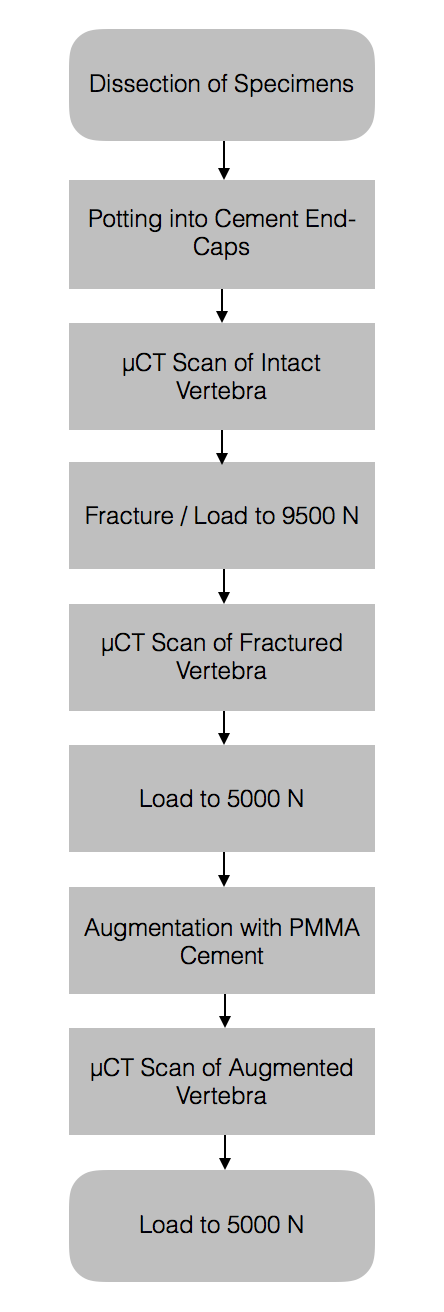
\includegraphics[width=2in]{images/Exp_FlowChart.png}
\caption{Flow-chart detailing the experimental process from initial dissection to final load test.}
\label{fig:exp_flowchart}
\end{figure}

\subsection{Specimen Preparation}\label{specimen-preparation-bov}

Bovine tails were acquired from a local abattoir and frozen to -20$^\circ$C prior to use.
They were defrosted
in a 4\(^\circ\)C fridge for approximately 24 hours before the
initial dissection. The three most caudal vertebral (CC1 to CC3) were kept,
discarding the remainder of the tail due to the elongation of the
vertebral body further distal of the first three vertebrae. In addition
to the elongation of the vertebral body the spinal canal narrows
limiting its ability to house a steel rod used for mounting the vertebrae in PMMA end-caps. Soft tissue was removed from the vertebrae as thoroughly as
possible, including the intervertebral disc material and material
occupying the spinal canal. This was carried out in order to remove
potential error when comparing experimental results of stiffness to the vertebra models developed from $\mu$CT scans (due to
difficulties modelling the soft tissues) and to allow a metal rod through
the spinal canal to aid alignment.


\begin{figure}[ht!]
\centering
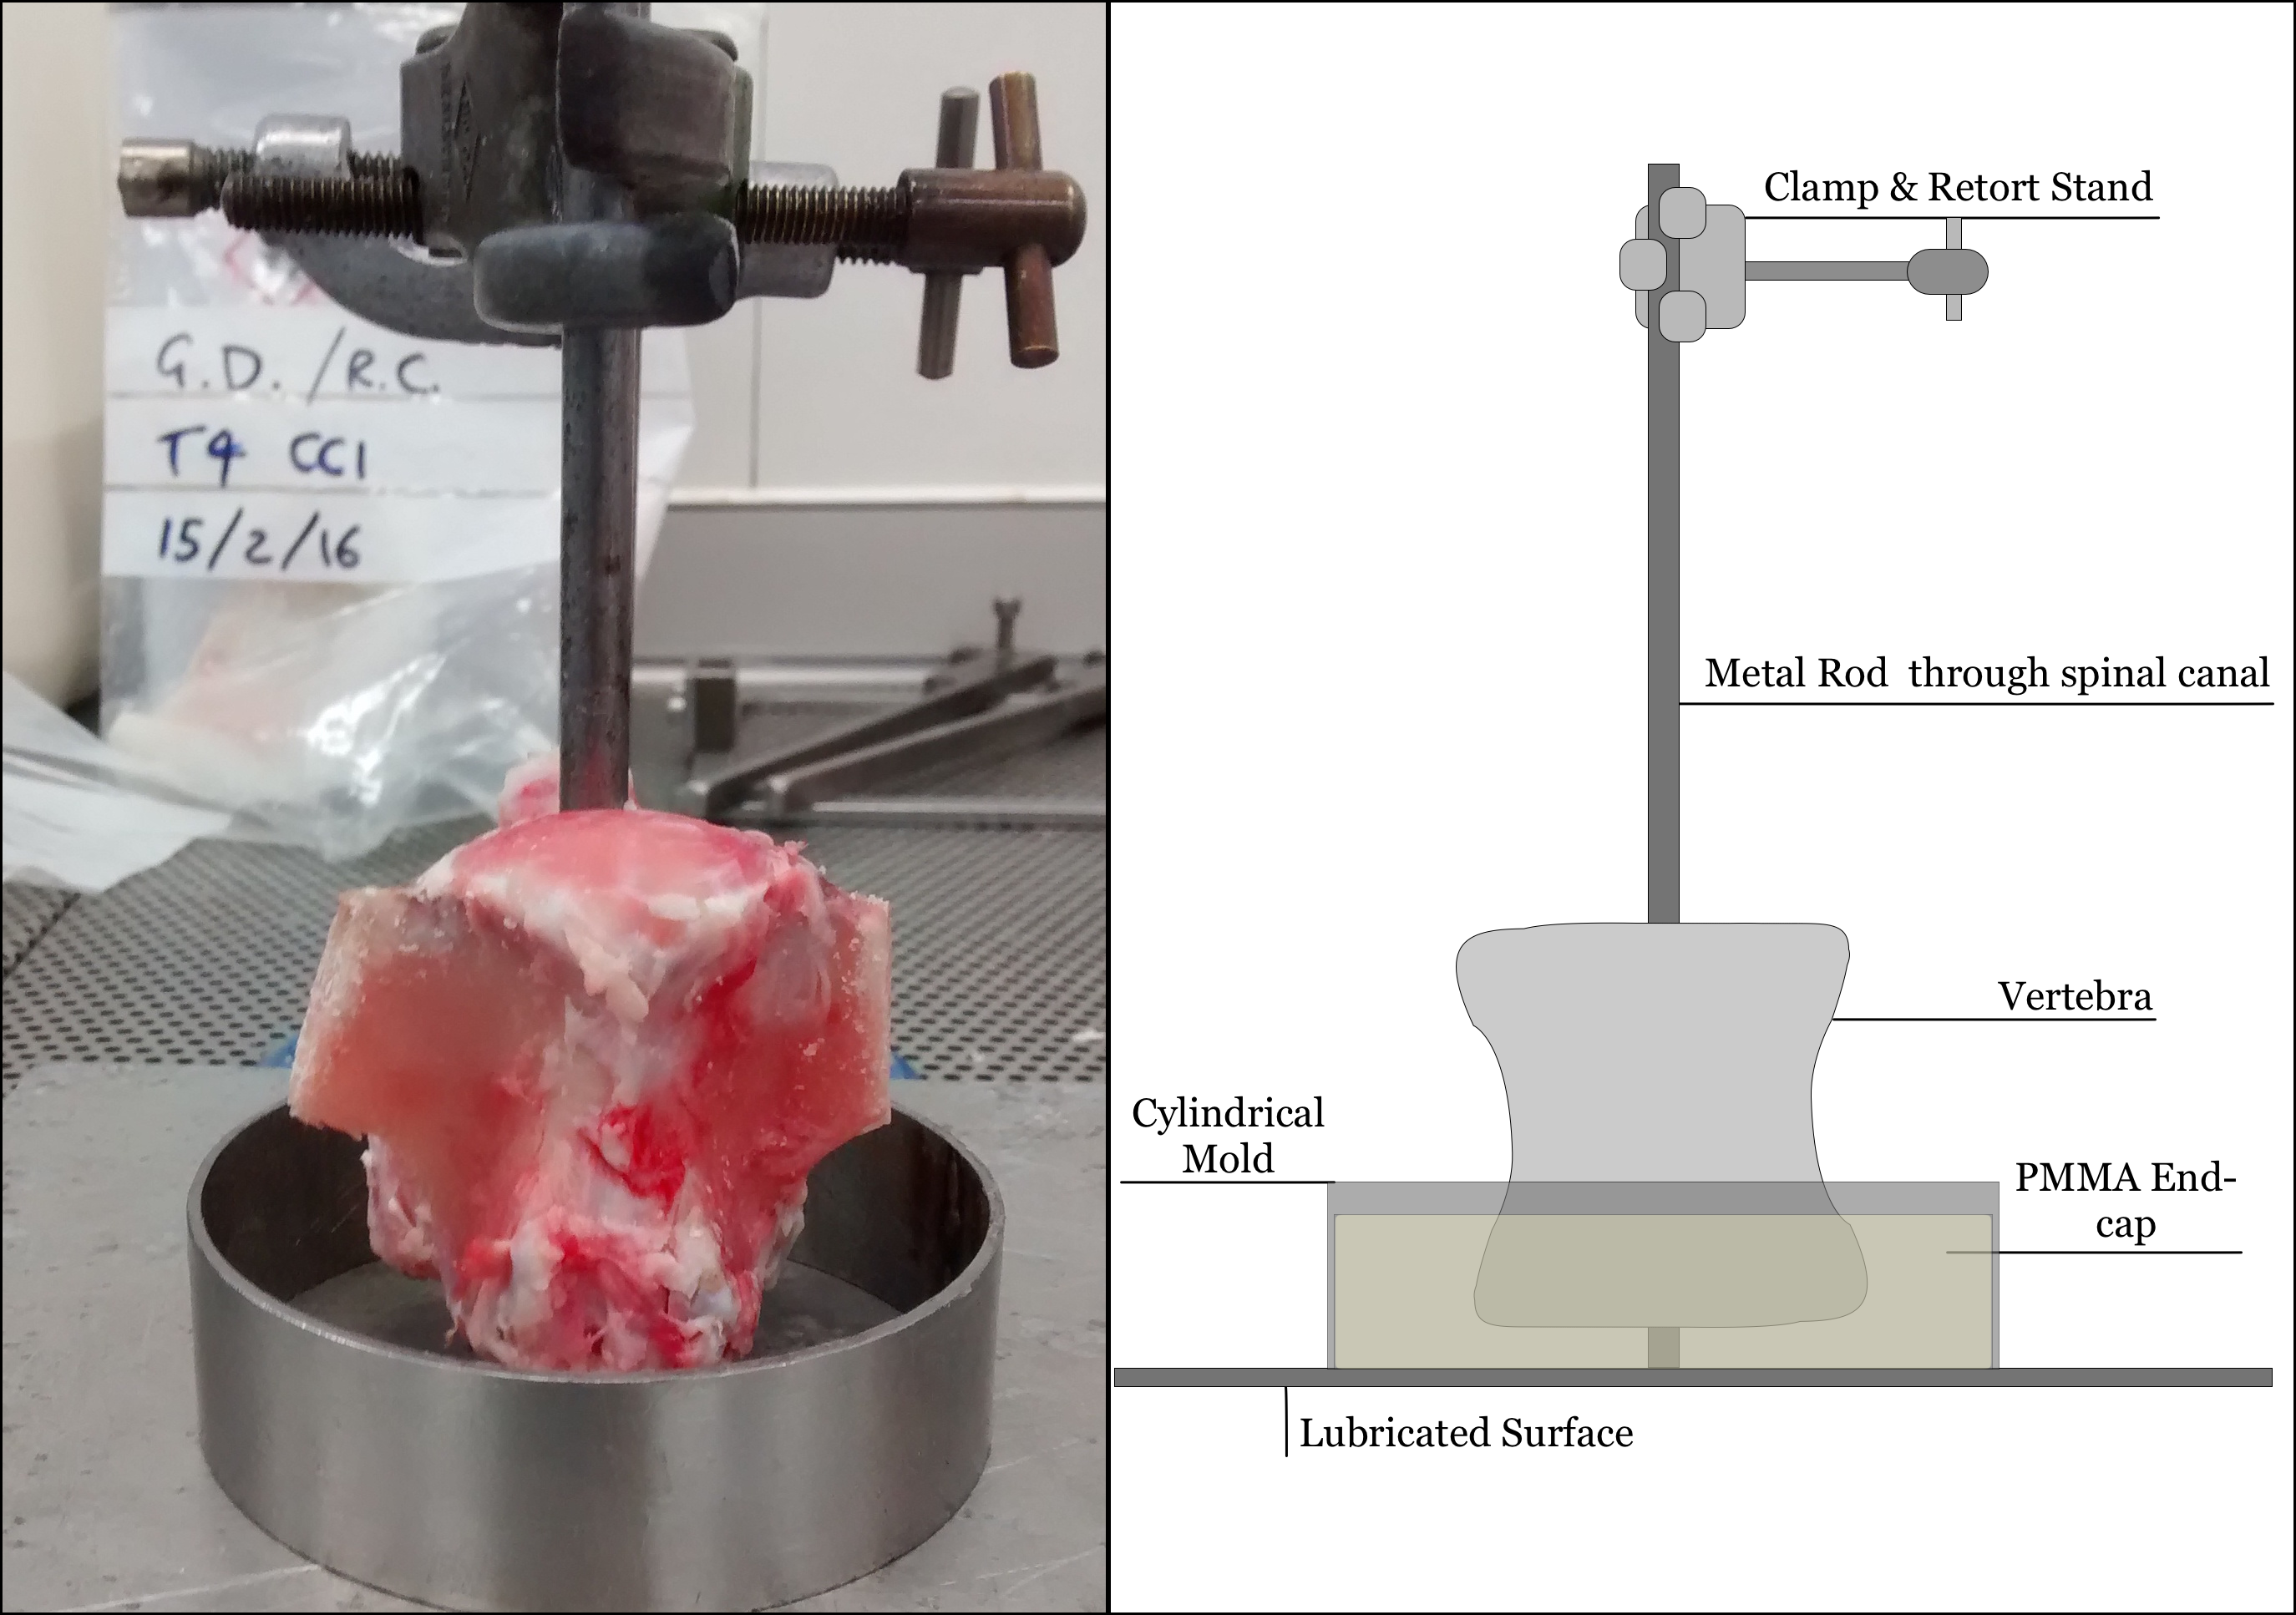
\includegraphics[width=5in]{images/potting_vertebra.png}
\caption{Photograph and diagram depicting the method of creating end-caps for the specimens.}
\label{fig:potting_vertebra}
\end{figure}



Once dissected (and in subsequent breaks between procedure steps) the
vertebrae were wrapped in phosphate buffered solution (PBS) soaked
tissue, in an attempt to limit the vertebrae from drying.
The specimens were potted in PMMA end-caps to allow repeated loading of the vertebrae with
the same orientation and positioning, while constraining the vertebrae
as little as possible and allowing flexion of the upper endplate. 
Such flexion (anterior and posterior loading), occurs naturally in the human spine, hence representing this experimentally is important.
The setup for potting the vertebrae can be seen in \cref{fig:potting_vertebra}.
Vertebrae were held using retort stands and clamps holding a rod placed
through the spinal canal. Depending on the level of the vertebrae the
spinal canal was packed with foam around the rod forming a snug fit
while the vertebrae was held approximately 5 mm above a petroleum jelly
lubricated metal surface. Also, depending on the level of the vertebrae,
any pedicles that protruded past the limits of the metal cylinders were
removed with a hacksaw at their base to prevent issues with the loading
and scanning tests which followed, most often this was limited to the
most caudal vertebrae and can be seen in \cref{fig:potting_vertebra}. Lubricated hollow metal cylinders of \(\sim\)10
cm diameter were used to form the endplate when the 2:1 powder to liquid
component PMMA mixture was added. PMMA was added until the endplate of
the vertebral body was covered up to the point where the body becomes
concave. After approximately 20 minutes the PMMA had sufficiently set to turn over
the vertebra and create the end-cap at the other end using the same
process with the addition of a level to ensure the creation of parallel
end-caps.

Once the PMMA was set the vertebrae were wrapped in more PBS soaked
tissue before being frozen or stored in a fridge until the vertebrae
were loaded to fracture. The specimens were frozen only if more than 24 hours
would pass before the next stage of testing to reduce the number of
freeze thaw cycles.

\subsection{Axial Compression}\label{axial-compression}

\subsubsection{Fracture Creation}\label{fracture-creation}

All specimens underwent axial compression using a material testing machine
in order to generate fractures within the vertebral body. Mounted
vertebrae were placed between two steel end-plates, the lower of which
contains four screws to inhibit lateral motion of the specimen when
under load and the upper plate contains similar screws, with the
addition of a chamfered hole. This chamfered hole allows the
alignment of the specimen so that the loading point was directly below
the head of the testing machine using the marker located above the centre of the vertebral body. The steel ball becomes the centre of rotation for
the free to rotate upper end-cap. This permitted rotation mimics natural
loading of the vertebrae and increases the likelihood of physiological
anterior wedge fractures. Details of the setup can be seen in
\cref{fig:expsetup}.

\begin{figure}[ht!]

\centering
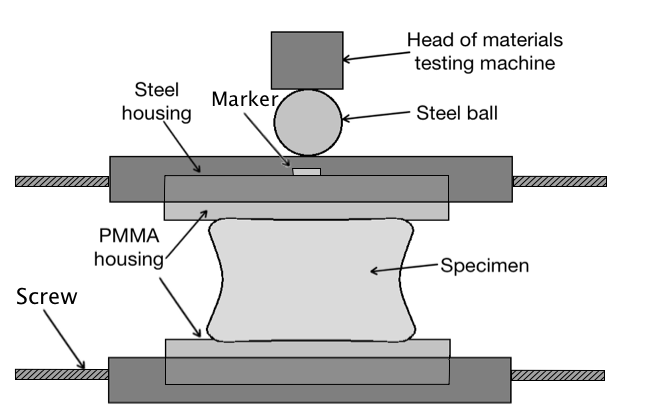
\includegraphics[width=3.68472in]{images/instrom_loading_diag.png}
\caption{The experimental setup for axial loading the vertebral
specimens.}
\label{fig:expsetup}
\end{figure}

Loading of the vertebrae starts with a preload from 50 N to 300 N for
10 cycles at a rate of 1mm/minute to remove any viscoelastic effects of any remaining soft
tissue. Following the preload, displacement was increased by 1 mm/minute
until either the load reached 9500 N (due to the 10 kN load cell limit)
or a visible failure occurred on the real-time load-displacement plot during compression.
This failure was observed as a peak in load with the compression being stopped once
clear decrease in load was observed. Both scenarios can be seen in \cref{fig:failure_non_failure}.



\begin{figure}[ht!]
\centering
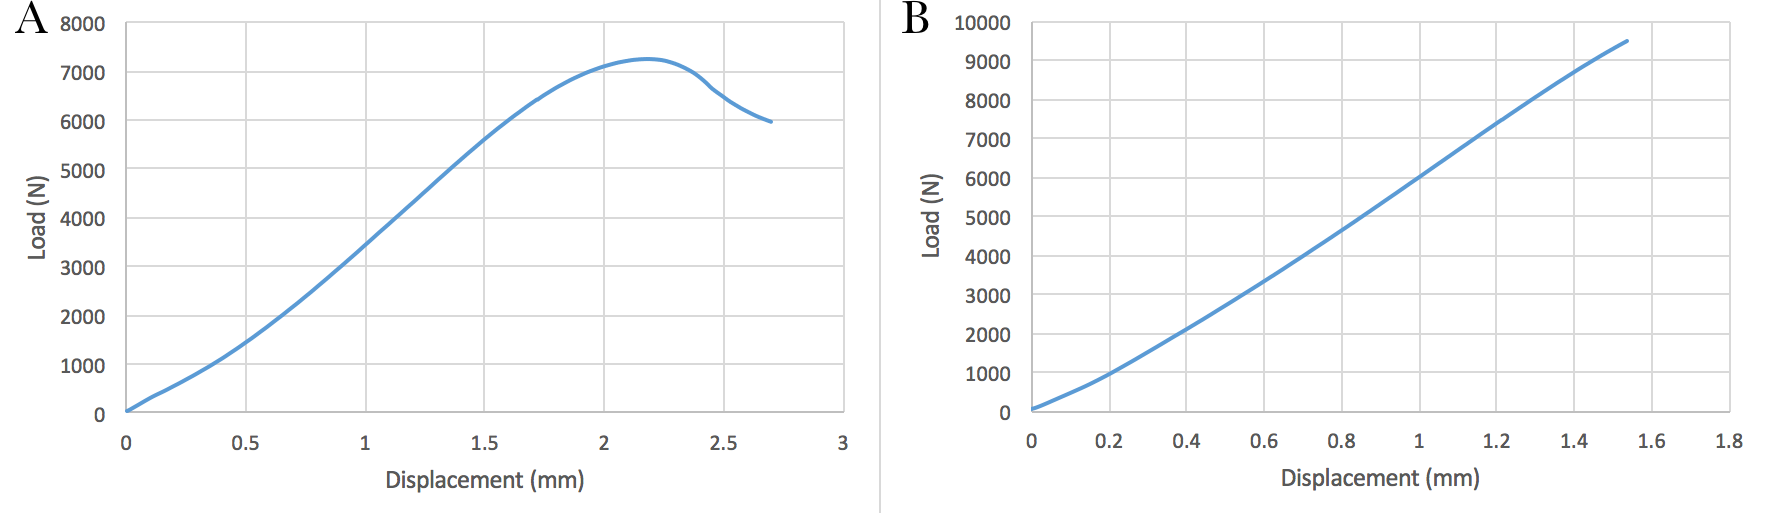
\includegraphics[width=16cm]{images/comparing_failureand_nonfailure.png}
\caption{The difference between failure (A) and non-failure (B) for bovine tail vertebra compressed to a maximum load of 9500 N or until a peak was observed.}
\label{fig:failure_non_failure}
\end{figure}

\subsubsection{Post Fracture \& Post
Augmentation Loading \& Stiffness
Calculation}\label{post-fracture-post-vertebroplasty}

In order to find the stiffness of the previously fractured and augmented
specimens a similar loading procedure was used. However, following the
preload, compression was stopped when the load reached 5000 N as a means
to limit additional damage and fractures to the vertebrae. This ensured that the vertebral stiffness across the three stages (intact,
post-fracture and post-augmentation) was calculated from the same range of loads (0 - 5000 N). To examine the effect that the initial load to failure has on the following loads, both post-fracture and post-augmentation, a control specimen was used. This control (T1 CC3) was only loaded up to 5000 N before ending the test.




%\begin{table}[ht!]
%\centering
%\caption{My caption}
%\label{my-label}
%\begin{tabular}{l|c|c|c}
%         & \multicolumn{3}{c}{Greatest Gradient (N/mm)}          \\ \hline
%Vertebra & \textless 1500 N & \textless 5000 N & \textless 9500 N \\ \hline \hline
%T8 CC1   & 4396.6           & 5914.3           & 6474.7           \\
%T8 CC2   & 7824.0           & 8132.8           & 8378.5           \\
%T8 CC3   & 3526.3           & 5680.6           & 6416.3           \\
%T9 CC1   & 4688.8           & 5833.5           & 6843.1           \\
%T9 CC2   & 3580.2           & 4449.8           & 4950.4           \\
%T9 CC3   & 3539.1           & 5093.7           & 5968.4
%\end{tabular}
%\end{table}

%add link to graph of load-disp showing wonky "linear region"

The stiffness of the specimens throughout their tests was calculated using a
Matlab (Mathworks) script on the raw data from the materials testing machine. The script was adapted from a script written by R. Coe (University of Leeds, 2016). The script
allowed the limits of the range of interest to be set and, using a defined
segment size, incremented over the data reporting the greatest stiffness found
in a segment. The segment size was set to 0.3 mm. The script iterated over the
data in overlapping increments of 0.1 mm and the range of interest was set to 0 - 5000 N, this can be seen in \cref{fig:load_disp_incr}.

\begin{figure}[ht!]

\centering
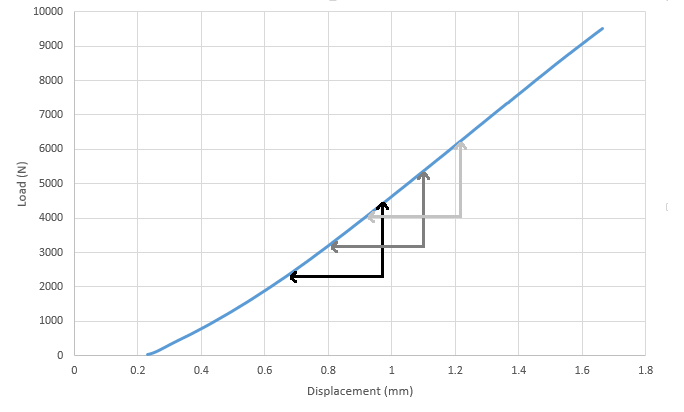
\includegraphics[width=4.18472in]{images/load_disp_incr.png}
\caption{A typical load displacement curve showing how the gradient was taken from 0.3 mm long sections incremented at 0.1 mm across the length of the curve.}
\label{fig:load_disp_incr}
\end{figure}

If the load-displacement curves were perfectly linear within the ``linear region" the stiffness in the three ranges of interest in \cref{fig:barchartcompgrads} would give an equal value for the stiffness or maximum gradient. However, given that these values were found to differ for the three ranges it suggested non-linear behaviour.
As shown in \cref{fig:barchartcompgrads} the recorded maximum stiffness varies greatly depending on what portion of the load displacement graph was being examined. The average difference between the 0 - 5000 N section and the 0 - 9500 N section was much smaller compared to the 0 - 1500 N section, hence 5000 N was used as the limit on the already fractured vertebrae tests. Due to the slight convergence towards 5000 N, this value was seen as a compromise between the risk of further damage whilst still obtaining a genuine value for the stiffness.


\begin{figure}[ht!]

\centering
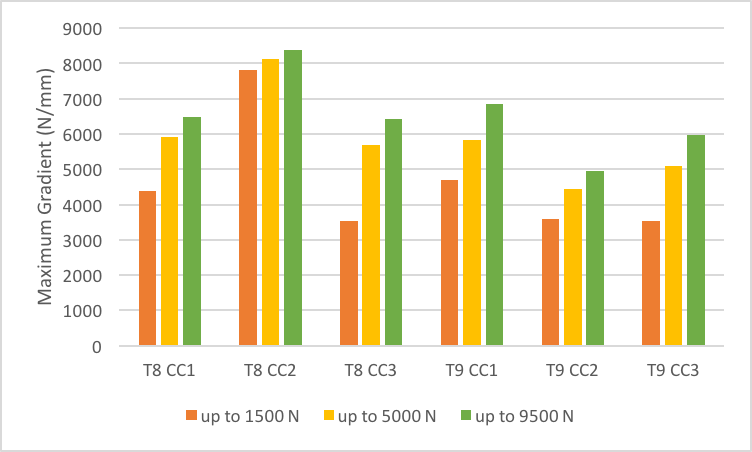
\includegraphics[width=4.18472in]{images/barchartCompGrads.png}
\caption{The difference seen when measuring the greatest gradient (stiffness) using different portions of the load displacement curve. From 0 to 1500 N, 0 to 5000N and 0 to 9500N.}
\label{fig:barchartcompgrads}
\end{figure}


\subsection{Vertebroplasty }\label{vertebroplasty-bov}
The procedure was developed in collaboration with two clinicians (Dr Peter Loughenbury \& Dr Vishal Borse) from the Leeds General Infirmary. Subsequent tests of the procedure were undertaken with the aid of Dr Sebastien Sikora, Dr Fernando Zapata Cornelio \& Ruth Coe (Research Fellow, Research Fellow \& PhD student respectively), while specimens with results presented here were augmented solely by the author.
Due to the differences between human and bovine vertebrae it was not possible to perform bi-pedicular vertebroplasty on the bovine specimens using the methodologies established for human vertebra.
The main difficulty was the greatly increased density of the bovine vertebra bone, meaning that rather than pushing the vertebroplasty needle into the vertebra by hand, a mallet and vice to hold the vertebra were required. In addition to this, the force required to inject cement into the vertebral body was greatly increased.
The vertebroplasty method for bovine tail vertebra was therefore developed over several iterations due to these difficulties. This sub-section details the initial procedure, the problems encountered and solutions developed to allow a clinically relevant volume of cement to be injected and captured in $\mu$CT scans.

\subsubsection{Initial Procedure}

The procedure was initiated by using bone nibblers to remove the rounded end of both posterior pedicles, providing a surface to start the needle entry. While holding the vertebra in a table mounted vice the needle's markings were used to estimate the depth and angle needed to reach the anterior quarter of the vertebral body. The placement of the needle required care to ensure the pedicle was not damaged through splitting as it was inserted. A mallet was used to insert the needle until it was at the depth
required; the procedure was repeated for the other pedicle, reusing the same needle.



The PMMA cement was mixed 1:1 monomer to powder to ensure that it could be drawn up via the syringe and to allow enough time to inject the cement before it thickened and set. This additional setting time and reduced viscosity is also used by clinicians, who use ratios up to 0.74 monomer to powder with no adverse outcomes associated despite the reduced modulus and strength often reported \cite{Belkoff2002,Jasper1999}.
While the vertebra was held in the clamp of a retort stand, the syringe was attached to the needle, which in turn was inserted into one of the pre-made tracks through the pedicle into the vertebral body.
%The syringe was then attached to the needle, with the interior rod removed, which was inserted to one side of the vertebra mounted using a retort stand.
Cement was pushed into the vertebrae using the syringe, until $\sim$3-4 mL was inserted into both sides of the vertebrae, with cement being used to back fill as the needle was removed. The vertebrae were then left for approximately an hour until the cement had set before scanning.

% Add picture and clarify


\subsubsection{Complications and Changes to the Procedure}\label{complications}

Various problems were encountered while carrying out the procedure that required the methods to be adapted. These challenges and their solutions are described below.

\paragraph{Vertebral Temperature}
The first of these was the difficulty found injecting any cement into the vertebra. With the initial specimens, cement was injected but it was mainly reserved to the needle tracks rather than the vertebral body. To counter this the vertebrae were warmed to 37$^\circ$C for an hour or until the internal temperature of the vertebrae had reached this temperature (using a temperature probe in the vertebroplasty needle hole). This meant that the bone marrow inside the vertebrae was no longer solid and therefore could be displaced by the cement making the injection much easier.

\paragraph{Radio-opacity of Cement}
A second problem was the opacity of the cement on $\mu$CT scans, which proved difficult to segment and separate it from the trabeculae in the vertebral body as can be seen in \cref{fig:withWithoutBaSO4}:A. Here, the cement was indistinguishable from the bone marrow and can only be seen in the needle channel. The solution to this was to mix barium sulphate (BaSO$_4$) with the PMMA to achieve the radio opacity seen in \cref{fig:withWithoutBaSO4}:B, where the bright area in the centre of the vertebral body is the injected cement and BaSO$_4$ combined. Due to the hydrophilic nature of the BaSO$_4$ powder it was important to use a completely dry beaker when thoroughly mixing it with the PMMA powder to limit aggregation of the BaSO$_4$, which can be seen in the bright spots in \cref{fig:withWithoutBaSO4}:B. The two components were used in a 1:4 BaSO$_4$ to PMMA powder ratio, mixed 1:1 with the liquid PMMA component.

\begin{figure}[ht!]
\centering
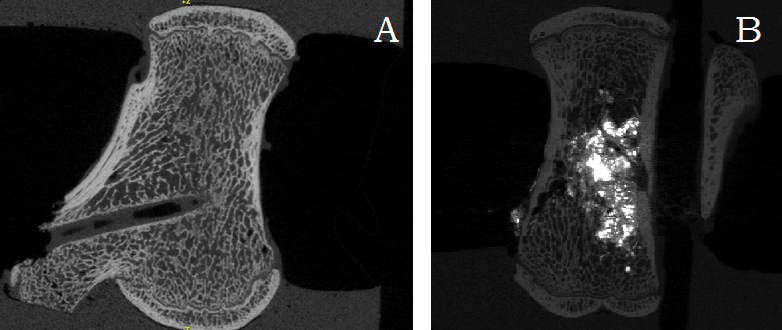
\includegraphics[width=4.18472in]{images/withWithoutBaSo4.png}
\caption{A: $\mu$CT scan of an augmented vertebrae, with some visible PMMA residing in the needle channel. B: $\mu$CT scan of an augmented vertebrae using PMMA mixed with barium sulphate.}
\label{fig:withWithoutBaSO4}
\end{figure}
\paragraph{Cement Leaking from Vascular Channels}
Preventing the cement from exiting the vertebrae from vascular channels while injecting the cement proved to be another obstacle to achieving a physiologic fill volume for the vertebrae. These channels lead both out the anterior face and from the vertebral body into the spinal canal, this can be seen in \cref{fig:cementleakage} and \ref{fig:2vertWithoutBluTac}. In the body these channels would be filled with vasculature preventing the cement leaking through them. Two main methods were used to stop cement leaking while carrying out the procedure on the bovine tail vertebra. The first was to use the same rod used for mounting the vertebrae in their end-caps to limit the passage of cement into the spinal canal. The second was to use blu-tac to cover the external vascular channels, wrapped with cling-film to hold it in place. This allowed any bone marrow free passage out of the vertebrae, but enough resistance to limit the flow of cement.

\begin{figure}[ht!]
\centering
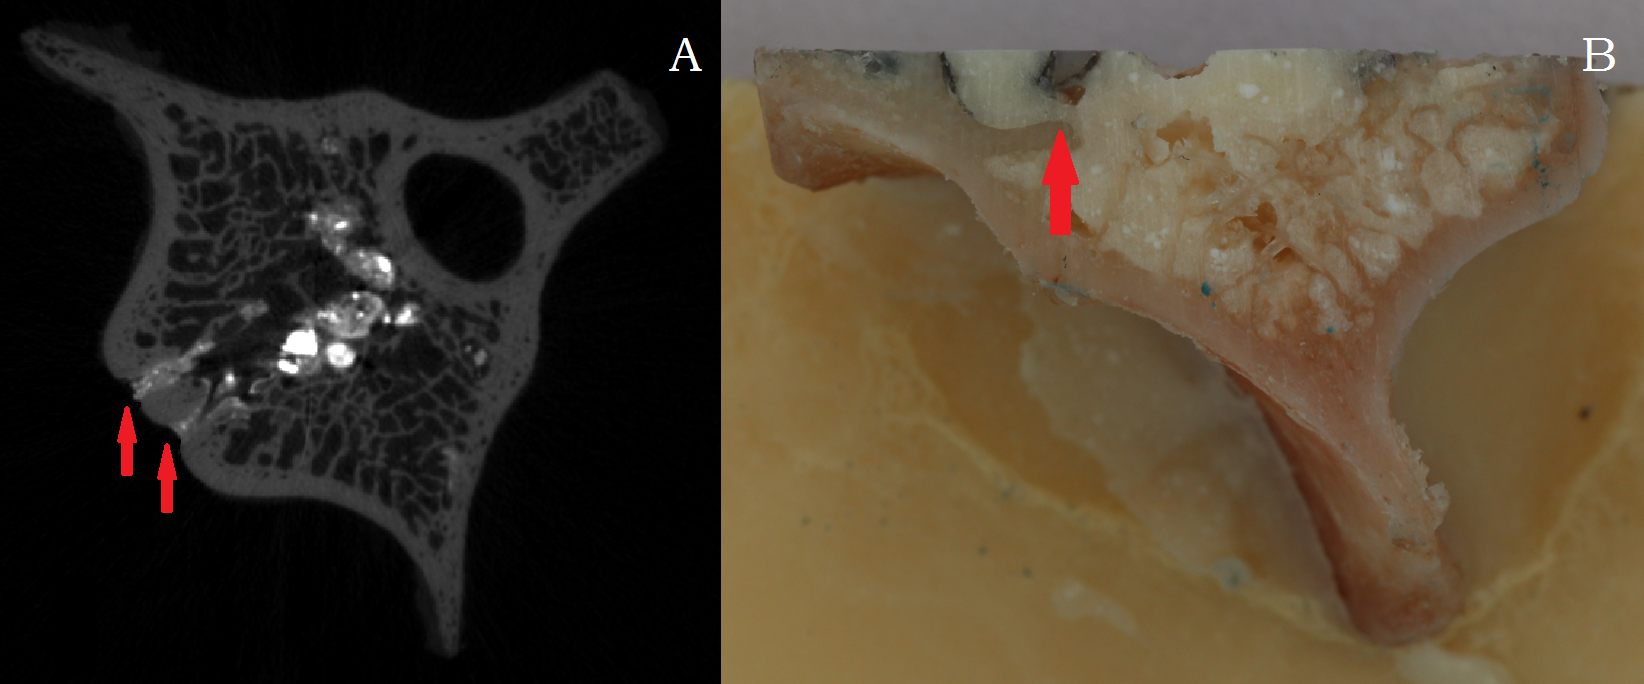
\includegraphics[width=4.18472in]{images/cementleakage.png}
\caption{A: $\mu$CT scan of an augmented vertebrae showing the cement leaking from vascular channels on the anterior side. B: Photograph of an augmented vertebrae cut into four quarters showing a vascular channel leading into the spinal canal.}
\label{fig:cementleakage}
\end{figure}

\begin{figure}[ht!]
\centering
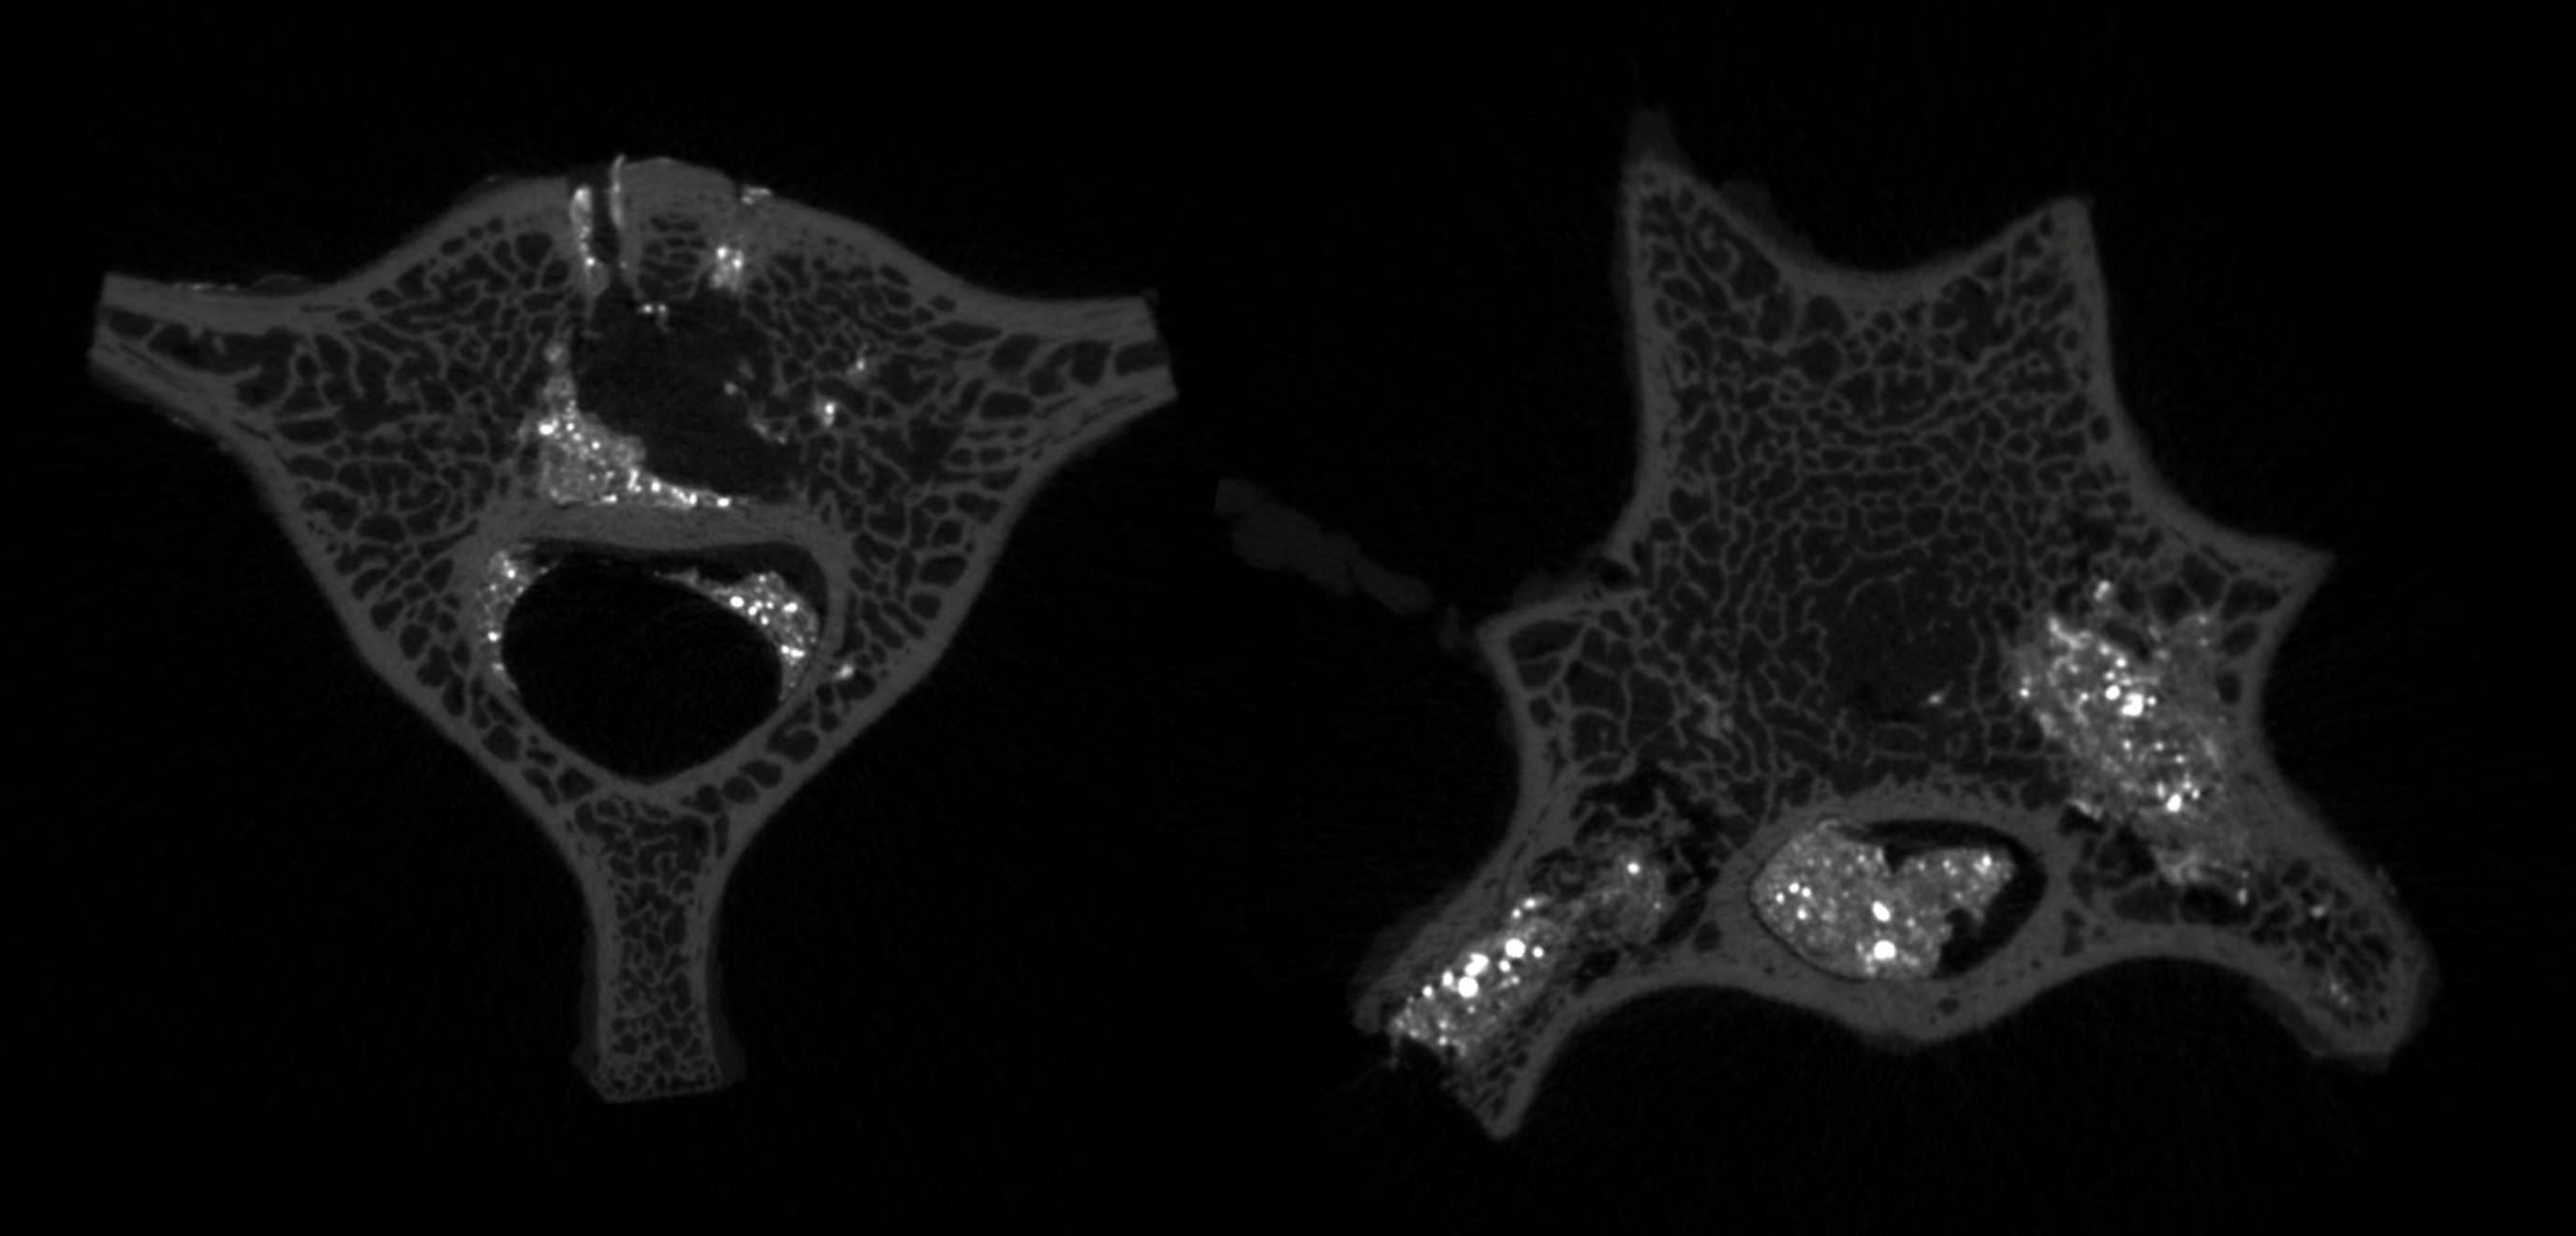
\includegraphics[width=4.18472in]{images/bigLeakage_noBluTac.png}
\caption{$\mu$CT scans of two vertebra, showing the cement leaking into the spinal canal and out of the vascular channels and the vertebral surface.}
\label{fig:2vertWithoutBluTac}
\end{figure}
% add figure of scan to make clear what the right hand pic is


\subsection{MicroCT Scanning}

$\mu$CT scans were taken at three occasions during the experimental process. These scans occur before and after the initial load to failure, then following the augmentation of the specimens. The process requires the vertebrae to be defrosted and at room temperature, given that the radio-opacity of water differs between solid and liquid states, hence vertebrae were usually defrosted overnight in a 4$^\circ$C fridge. Vertebrae were loaded two at a time in a carbon fibre loading cradle designed for the HR-pQCT (XtremeCT, Scanco Medical AG, Switzerland) scanner. The settings used for the scans were: an isotropic voxel size of 82 $\mu$m, energy settings 900 $\mu$A, 60 kVp and 300 ms exposure time.

\subsection{Results}\label{results}

The stiffness values for 12 bovine tail vertebra from the first to third vertebra down, shown in \cref{fig:allexpData}. Of the twelve vertebra only two, the first and second tail vertebra of the second tail (T2 CC1 \& T2 CC2), were fractured. The remaining nine (excluding T1 CC3, the control) reached 9500 N and therefore did not fail. It is also difficult to see whether the initial load to failure had any effect on the subsequent loads. This is mainly due to the lack of control specimens and the large variation of results in general following the first load.

\begin{figure}[ht!]
\centering
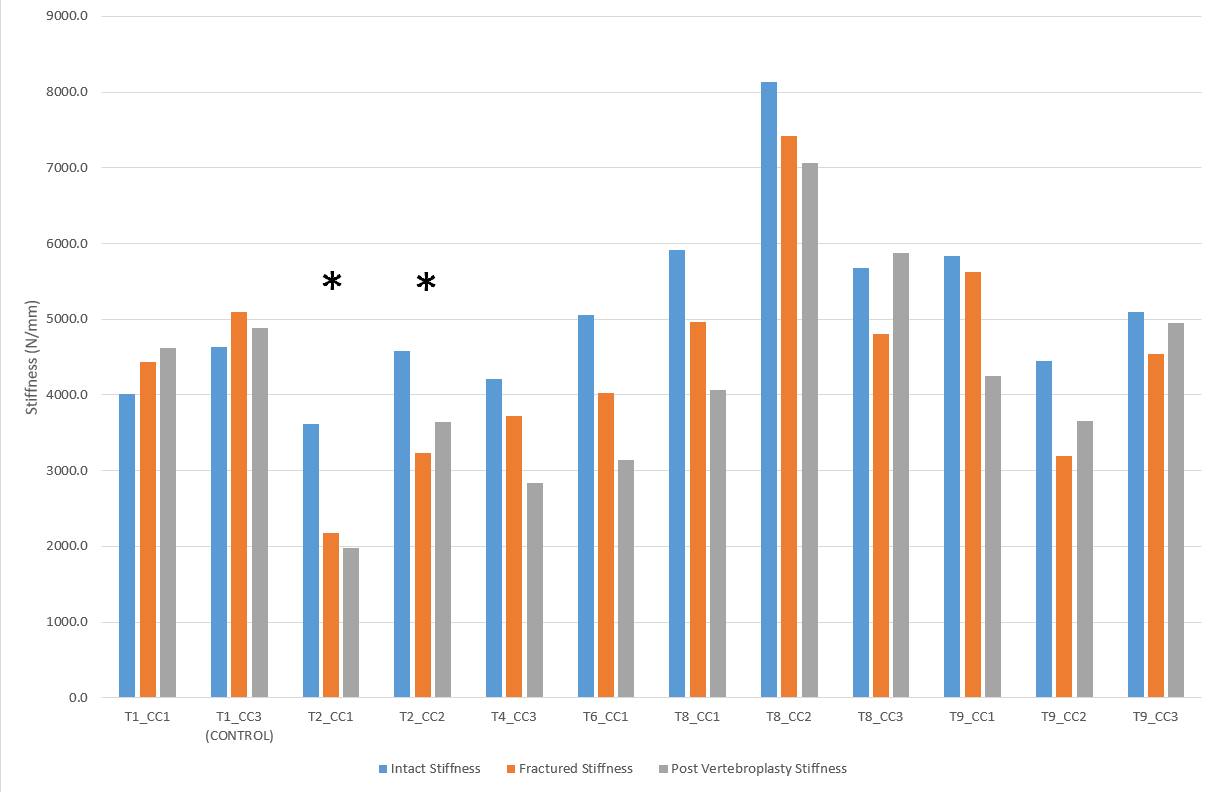
\includegraphics[width=\textwidth]{images/All_experimental_Data.png}
\caption{The maximum stiffness of 12 bovine tail vertebrae between 0 and 5000 N taken from load - displacement data. Showing the stiffness of the intact vertebrae, a post - fracture stiffness and a post - vertebroplasty stiffness for each. * Indicates those specimens that achieved a clear failure below 9500 N.}
\label{fig:allexpData}
\end{figure}

The results for the fill volume of cement in the augmented specimens is presented in \cref{tab:cementVol} and was acquired from the down-sampled, segmented models generated from $\mu$CT scans. It shows that fill volume varies between 3\% and 17\% fill and in addition shows a lack of a correlation between fill volume and increase in augmented specimen stiffness over fractured stiffness. \cref{fig:t2CC2vsT8CC2} shows the extent of the cement fill for the two vertebrae with the largest fill volume.

\begin{table}[ht]
\centering
\caption{The volume of cement and the vertebra volume for the 12 specimens used, along with the percentage cement fill and an indication as to whether the stiffnesses of the augmented vertebrae were greater than the fractured stiffness. This information was measured from the down-sampled models generated from $\mu$CT scans of the vertebrae.}
\label{tab:cementVol}

\begin{tabular}{l|>{\centering\arraybackslash}p{\dimexpr.16\textwidth}>{\centering\arraybackslash}p{\dimexpr.16\textwidth}>{\centering\arraybackslash}p{\dimexpr.16\textwidth}>{\centering\arraybackslash}p{\dimexpr.24\textwidth}}
Vertebrae & Cement Volume (mm$^3$) & Vertebra Volume (mm$^3$) & Cement Percentage of Vertebra Volume (\%) & Increase in Augmented Stiffness over Fractured Stiffness \\
& & & & \\ \hline \hline
T1 CC1 & 2260 & 32440 & 6.97 & * \\
T1 CC3 & 465 & 27039 & 1.72 &  \\
T2 CC1 & 663 & 23285 & 2.85 &  \\
T2 CC2 & 3405 & 20373 & 16.71 & * \\
T4 CC3 & 1363 & 25446 & 5.36 &  \\
T6 CC1 & 830 & 29332 & 2.83 &  \\
T8 CC1 & 1257 & 37357 & 3.36 &  \\
T8 CC2 & 4489 & 29248 & 15.35 &  \\
T8 CC3 & 1041 & 28403 & 3.67 & * \\
T9 CC1 & 2922 & 45681 & 6.40 &  \\
T9 CC2 & 2210 & 38894 & 5.68 & * \\
T9 CC3 & 2437 & 35840 & 6.80 & * \\ \hline
\end{tabular}%
\end{table}

\begin{figure}[ht]
\centering
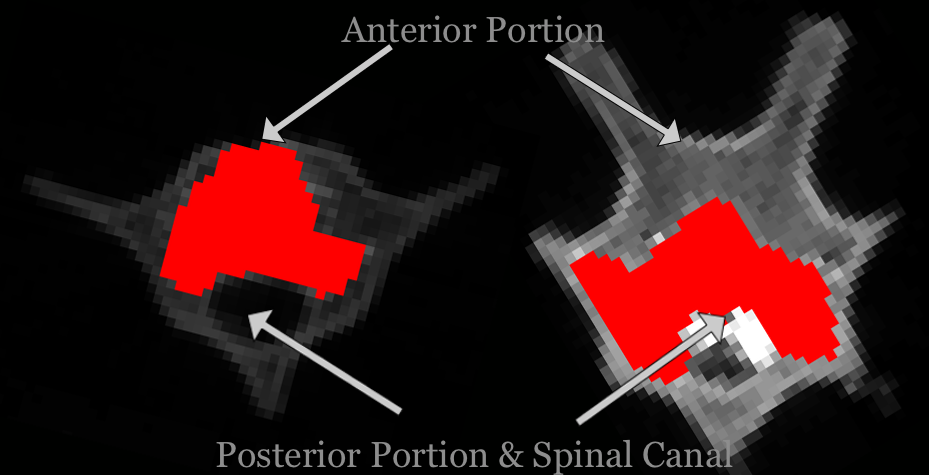
\includegraphics[width=4in]{images/t2CC2vsT8CC2.png}
\caption{$\mu$CT scans of T2-CC2 (left) and T8-CC2 (right), with cement masked in red, showing the extend of cement fill at the point where the cement was most anterior. }
\label{fig:t2CC2vsT8CC2}
\end{figure}

The attempt to reduce cement leaking through vasculature during the vertebroplasty procedure can be seen in \cref{fig:4vert_withBlutac}. The methods employed greatly reduced the the quantity of cement observed in both the spinal canal and around vascular channels at the vertebral body surface when compared to scans in \cref{fig:2vertWithoutBluTac}.

\begin{figure}[ht!]
\centering
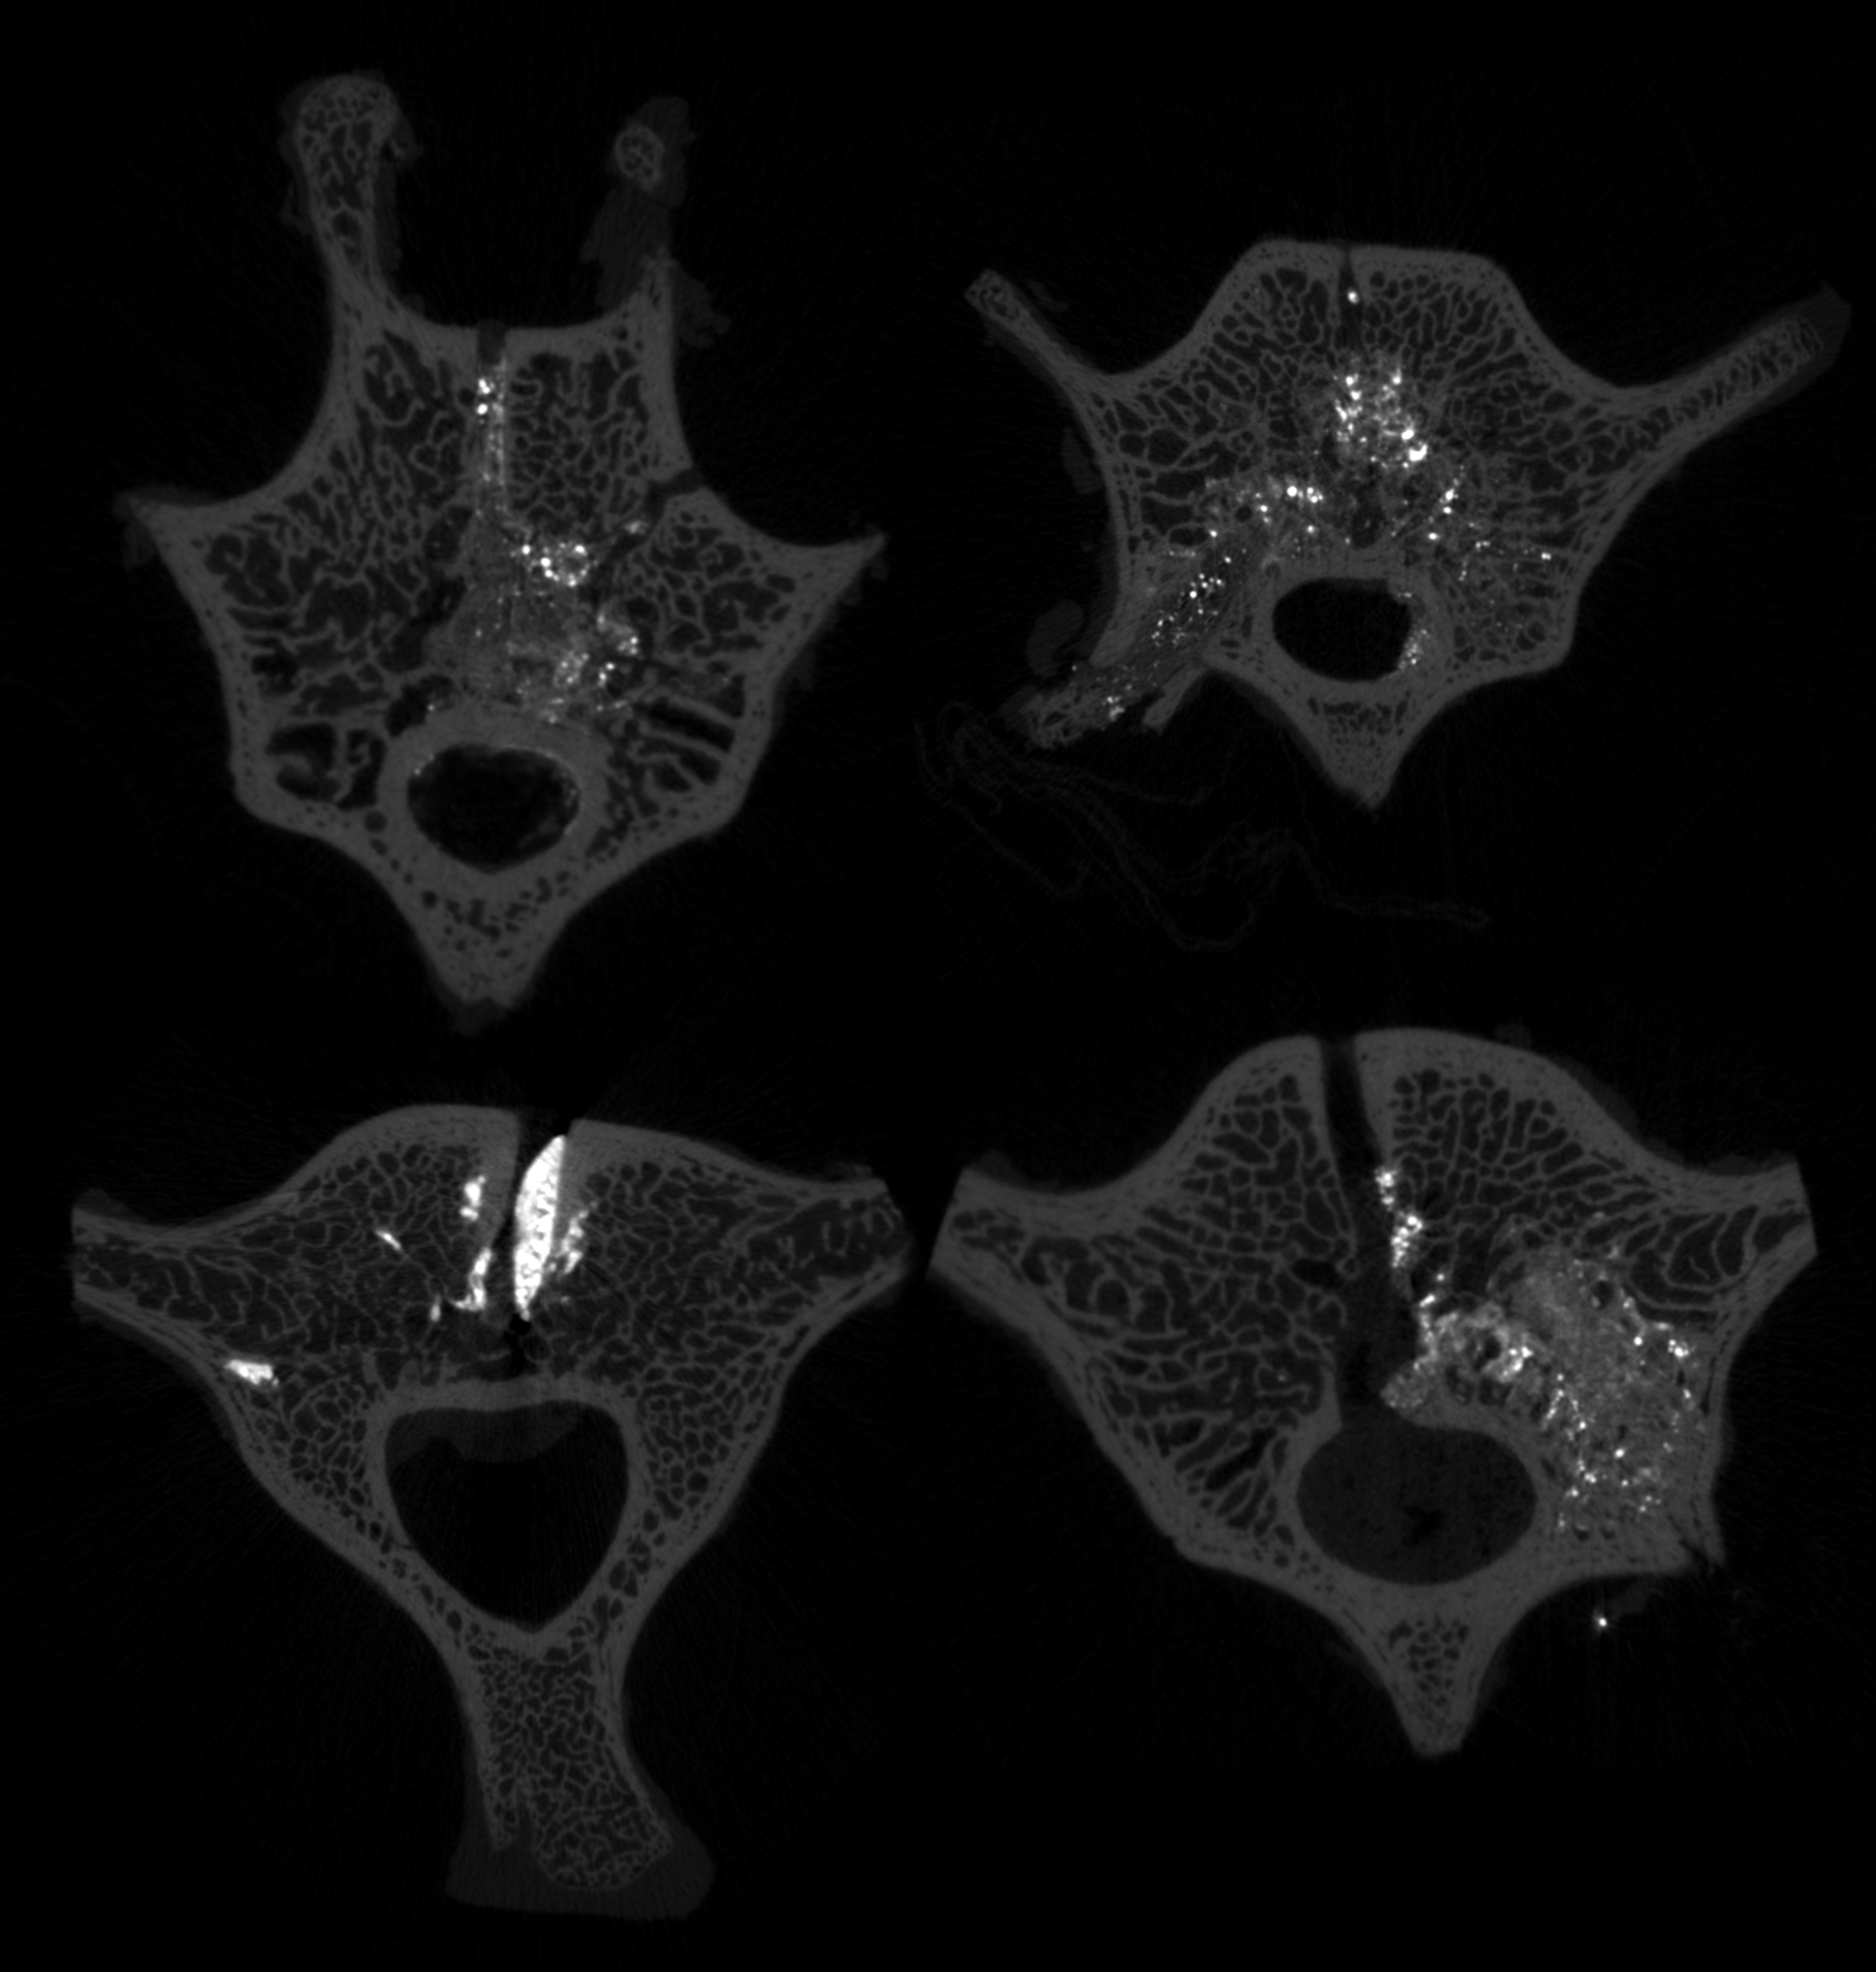
\includegraphics[width=3.8in]{images/4vertPostBluTac.png}
\caption{$\mu$CT scans of four augmented vertebra using a steel rod to fill the spinal canal and blu-tac to cover the external vascular channels. Shows greatly reduced cement content within the spinal canal with less cement at the surface of vascular channels.}
\label{fig:4vert_withBlutac}
\end{figure}


The two plots in \cref{fig:deltaStiffness_Vs_intact} show a lack of correlation between the difference in stiffness after augmentation when compared to both the fractured and intact specimen stiffness and the intact stiffness. Showing that magnitude of any increase or decrease in the vertebral stiffness following augmentation is not caused, or a feature of the initial, intact vertebral stiffness.

\begin{figure}[ht!]
\centering
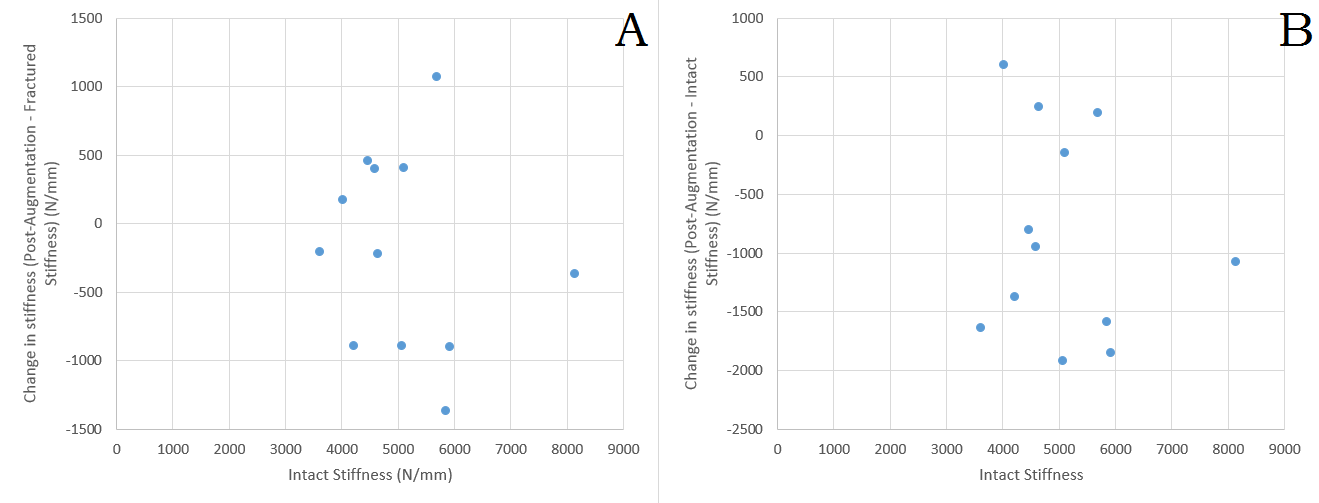
\includegraphics[width=\textwidth]{images/deltaStiffnessVsIntact.png}
\caption{A: The difference between the post augmentation and fractured stiffness against the intact stiffness. B: The difference between the post augmentation and intact stiffness against the intact stiffness.}
\label{fig:deltaStiffness_Vs_intact}
\end{figure}

\subsection{Discussion}\label{discussion-bov}

The experimental work carried out so far provides a good basis for both the continued modelling of vertebroplasty (especially modelling the cement - trabecular interface which is discussed in later sections) and to continue the experimental work using human tissue. Understanding the challenges of vertebroplasty (those discussed above), will be invaluable when transitioning onto the much more limited sou nrce of human vertebrae.

%^ reiterate aims of exp work

Regarding the results of stiffness at the intact, fractured and augmented stages, the expected trends were not always clear. Most commonly the intact vertebrae have the greatest stiffness with the fractured stiffness showing a reduced value following the damage created with the initial load to failure. The variation of the decrease (and increase) in stiffness for the fractured vertebrae may have a variety of reasons, although the most likely cause is level of damage caused in the initial ``load
to failure''. These tests varied between the typical load displacement that includes a failure (\cref{fig:failure_non_failure}:A) and those that show no sign of failure up to the limit of the load cell (\cref{fig:failure_non_failure}:B). It is difficult to observe any correlation between these vertebra that showed clear failure (T2-CC1 and T2-CC2), those that reached 9500 N and a reduction in the fractured stiffness. It is not to say that the vertebra that reached 9500 N experienced no damage, with the gradient of the load displacement curve often reducing and plateauing as the 9500 N limit approached. The interesting increase in the fractured stiffness for T1-CC1 compared to the intact stiffness may be explained if it is assumed that the compacted trabeculae following the first load to 9500 N result in a stiffer material for the following tests.

The cement fill volume information shows that a small percentage of cement is injected into the vertebrae on average, with only two vertebrae approaching the clinically relevant 20\% fill. Unexpectedly, only one of these two vertebrae showed an increase in augmented stiffness over the fractured stiffness. A possible explanation is that it is not only the fill volume that is important in restoring the vertebral stiffness but the placement too. This is shown when comparing the segmented scans of the the two vertebrae with the greatest fill volume with the T2-CC2 specimen showing cement extending to the anterior wall of the vertebral body, while the cement is limited to the posterior and centre of the vertebral body for T8-CC2. This may help to explain why the stiffness of T8-CC2 did not increase following augmentation. The reduction in stiffness following augmentation for seven of the twelve vertebrae may be due to damage caused by the insertion of vertebroplasty needles. Clinically this damage left behind from the needle channels would heal, most likely restoring the stiffness of the vertebrae back to its intact properties.

Another possible area of inconsistency is the temperature at which the vertebra were mechanically tested, while it is ensured that the specimens were fully defrosted they were tested at both fridge temperature (4$^\circ$C) and room temperature (20$^\circ$C). The effect of this variation in temperature needs to be identified and depending on the results more closely monitored.

Despite encouraging results regarding the vertebroplasty methodologies it was difficult to achieve the desired quantity of the cement in the vertebral body. This was mainly due to the difficulty injecting the cement in a smooth manner, which may have been caused by either the tip of the needle becoming blocked following its reinsertion into the needle track, more viscous marrow stopping the displacement of less viscous marrow by the cement or compacted trabeculae around the needle channel that limit the flow of cement past them. One option to test in future work would be side opening needles, which would help guide the cement more accurately to the regions required while circumventing issue with the needle becoming blocked.

The experimental methods currently developed will be of great value when starting experimental work using human tissue albeit many will require adaption due to the differences between the tissue types. These include the density of the bone and methods of inserting the needles, where with the available human tissue being from the elderly, the bones will be most likely be osteoporotic. These bones will require more care to reach the correct region of the vertebral body with the needle and to ensure a clinically relevant volume of cement is used.


%Talk about extra plots in results - deltaStiffness and cement fill.

\pagebreak

\section{Finite Element Modelling
Methods}\label{finite-element-modelling-methods}

The aims of the finite element section of work were to develop methods that enable the creation of specimen specific models of vertebrae (both bovine tail and human). Initially the focus was on the generation of models that accurately describe the mechanical behaviour of intact bovine specimens, once this was achieved an attempt to model augmented specimens was made. In addition to these larger goals, certain sensitivity tests were carried out, including those to understand the effects that additional meshes have on model stiffness.

%^ introduction paragraph

\subsection{Model Creation}\label{model-creation}

The computational analyses of linear-elastic finite element models is
carried out using a combination the segmentation and meshing software, ScanIP (Simpleware, Exeter, UK) and the simulation software, Abaqus (Dassault Systemes, France). The $\mu$CT scans were converted into a
finite element mesh using the former software package, this was then
imported into the second piece of software to be configured and solved.

The scans acquired from the \(\mu\)CT scanner were converted from the ISQ
file format, generated by the scanner software, into the more portable TIFF image format files using an existing in-house  matlab script that
additionally converts the greyscale of the scan into 256 bins. This conversion from 16 bit TIFF files with 65,536 bins to 8 bit TIFF files was required due to the limitation to 255 material properties within Abaqus, this allows one greyscale value per material property (assuming all 255 greyscale values are represented in the scan). Once the
scan has been pre-processed it was imported into ScanIP ensuring
that the spacing of voxels was correctly set - in this case 82 \(\mu\)m.
Once imported, the location of the loading point was identified to
simulate the correct experimental load within ABAQUS; the marker (see \cref{fig:expsetup})
appears bright on the scan and its centre was taken as the load point,
calculated by converting the position into mm. This was achieved by
multiplying by the native resolution of 82 \(\mu\)m.

The following parts of model creation were carried out using a Python script from within the ScanIP software. The script carries out the process described below and was generated by the author by carrying out the process manually and in order to understand the steps required and then writing a script to perform those actions. The development of the script removed much of the user variation in the segmentation of each vertebral model.

\begin{figure}[ht!]
\centering
  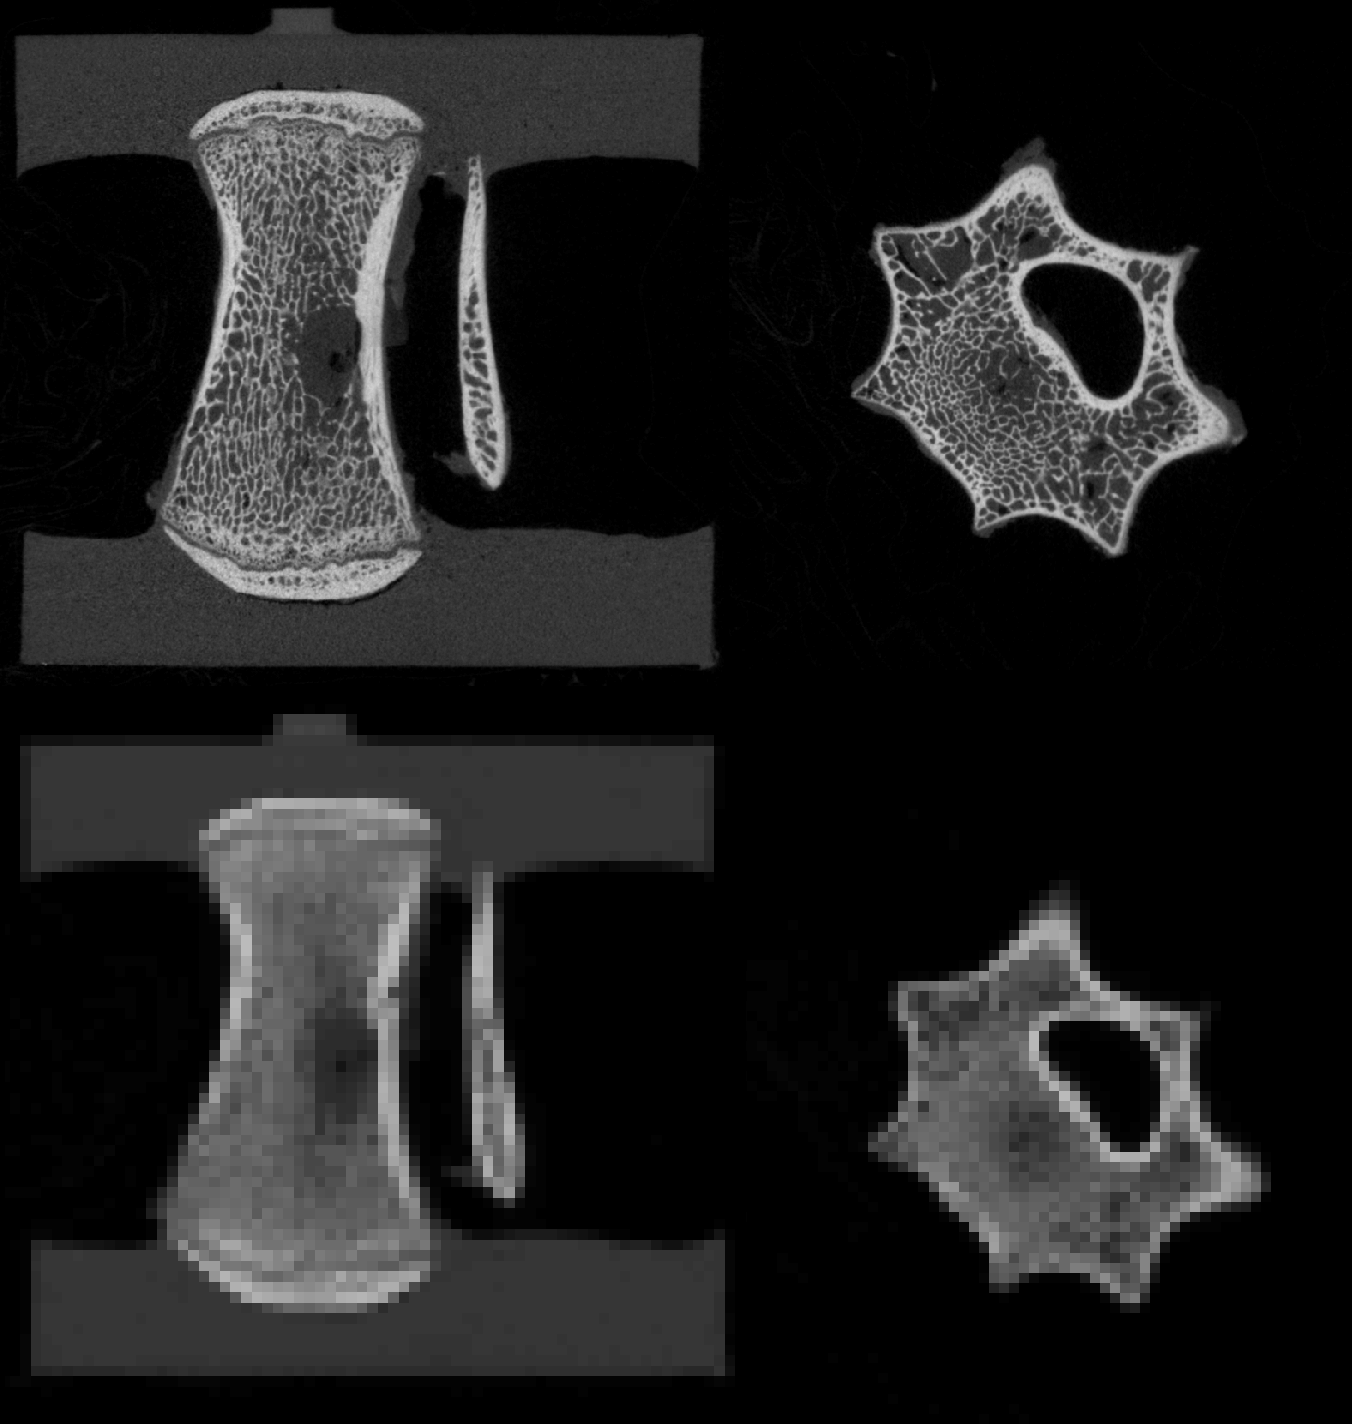
\includegraphics[width=4in]{images/compofDownsample.png}
  \caption{Side and top view of a vertebral $\mu$CT scan showing the effect of the downsample from 82 $\mu$m to 1mm cubed.}
\label{fig:compofDownsample}
\end{figure}




It was easier to down-sample the image stack prior to
segmentation, due to the time required for the software to generate
high resolution masks and increased memory usage at higher resolution. The effect of down-sampling can be seen in \cref{fig:compofDownsample}. However, in certain cases, for example when
modelling vertebral augmentation, in order to attempt to capture the
intricacies of the structure and the boundaries between cement and
trabecular bone it was favourable to generate the mask prior to down
sampling, \cref{fig:fullressVPseg}. The image stack was down-sampled to voxels 1 mm cubed, due to
previous studies producing sensitivity to mesh size results that showed
a good trade off between computational cost and model accuracy \cite{Jones2007}.



\begin{figure}[ht!]
\centering
  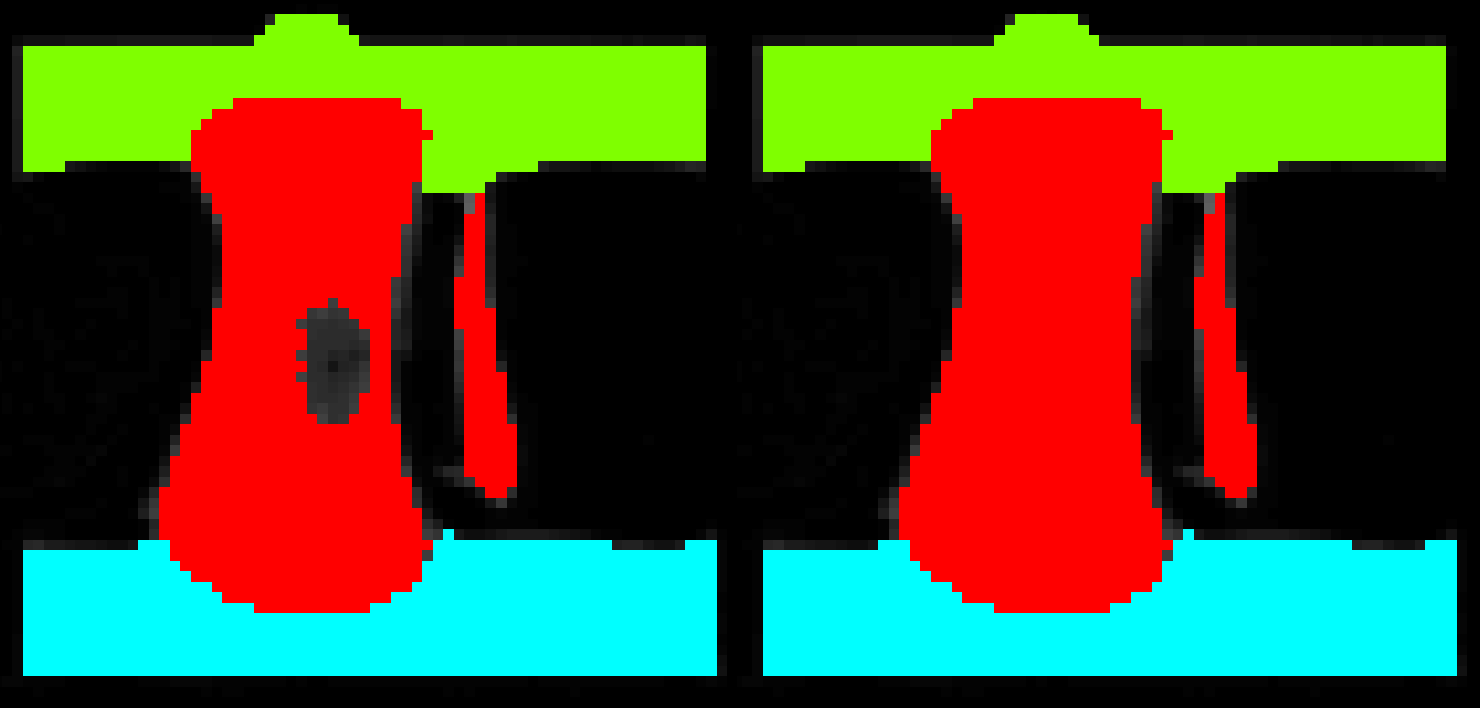
\includegraphics[width=4in]{images/fillTheVoid.png}
  \caption{Side view of a vertebral model showing segemented vertebra, including the internal void that is filled.}
\label{fig:fillTheVoid}
\end{figure}


Once down-sampled the image stack was segmented into the constituent
parts - the vertebrae and cement end-caps. The different regions that
were required to be segmented have different greyscale values, hence the
general shape of the masks was created through a thresholding tool that
selected volumes of the image stack between two bounds. For the end-caps
these bounds were usually between greyscale values of 12-22 and, if the
specimen was not augmented, the vertebrae between 23-255. For augmented
specimens these limits change to 23-65 for the vertebrae and 66-255 for
internal cement containing barium sulphate. These values were selected by visually limiting the amount of unwanted material selected within the threshold and maximising the wanted material, for example - selecting as much of the end-caps as possible while limiting the selected background and vertebral material to a minimum. This thresholding can be seen in \cref{fig:fillTheVoid}.
 It was preferable to avoid
internal voids within each mask, due to the potential for errors that
can be thrown once the model is imported into ABAQUS, these were
removed with the use of the morphological close and cavity fill tools within ScanIP (\cref{fig:fillTheVoid}).





The following parts of the method were carried out manually, following the completion of the automatic segmentation python script. The two end-caps were separated into two
separate masks by first duplicating the mask and then flood filling each end-cap to form separate masks.

An FE model was created using the previously generated masks and properties for the volume meshing, materials and contacts were set. The grid size for the model was set to 1 $\times$ 1 $\times$ 1 using the FE grid algorithm which uses a mix of tetrahedral and hexahedral elements. Material properties were set to homogenous with a density = 1, Young's modulus = 2.45 (GPa) and Poisson's ratio = 0.3 for the end-caps and when appropriate, were set to the internal cement volume. The material
properties for the vertebral volume were set to a greyscale based material type using the greyscale background information. The coefficients were set so that both the density and Young's modulus were equal to the greyscale value for that element, allowing the Young's modulus to be set correctly in following steps and as described in Section \ref{material-properties-bov}.

Contacts were set as placeholders to be edited in Abaqus in the steps following. These were contact pairs between each component and another between the superior end-cap and the upper boundary on the Z-axis. The second contact type was a node set between the inferior end-cap and the lower boundary on the Z-axis.

\begin{figure}[ht!]
\centering

  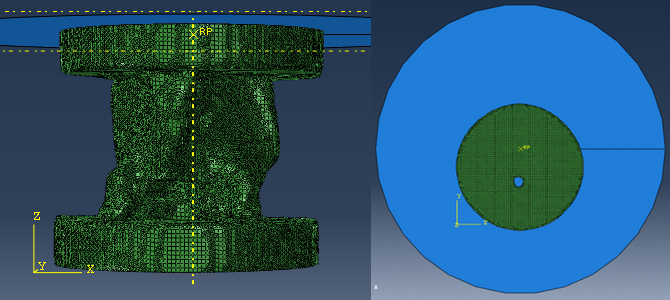
\includegraphics[width=4in]{images/abaqus_side_view_Both.png}
  \caption{Side \& top down view of a vertebral model showing the alignment of the analytical rigid plane.}
\label{fig:abaqus_top_view}
\end{figure}


Following this, the FE model was meshed, then exported into an INP file format. The model was then imported into Abaqus where the following configuration was completed by a second python script. An analytical rigid plate was created to represent the upper loading platen of the materials testing machine and was centred at the loading point previously found from the marker, this can be seen in \cref{fig:abaqus_top_view}. Once aligned any previous placeholder interactions were removed and a tied interaction was created between the rigid plate and the superior end-cap, along with tied interactions between the vertebra and both end-caps and, if appropriate, to the internal cement volume. An encastre boundary condition was created at the bottom surface of the inferior end-cap removing all rotational and translational movement and therefore mimicking the experimental setup. A displacement boundary condition was applied to a reference node at the centre of the rigid plate and therefore loading position, the properties were set such that 1 mm of displacement occurs in the negative Z direction; lateral motion in the X and Y planes was restricted, while rotation about the loading point was allowed - again mimicking the experimental setup.

The python script was written to set the material properties of the greyscale dependant vertebral elements by setting the Young's modulus to the greyscale value multiplied by a conversion factor (which is discussed in section \ref{material-properties-bov}). The script allowed Abaqus to solve the models and outputs the stiffness for each model. This was calculated by the dividing the axial reaction force (axis of load application) at the reference point by the displacement at 1 mm of displacement.

\subsubsection{Augmented Model Generation}

In order to attempt to capture the detail of interdigitation between the
vertebrae and the injected cement, the masking process was carried out prior to downsampling, seen in \cref{fig:fullressVPseg}. If masked post-down-sample it became difficult to define the cement boundaries and the masked volume was inaccurate when compared to the full resolution scan.


\begin{figure}[hbt]
\centering

  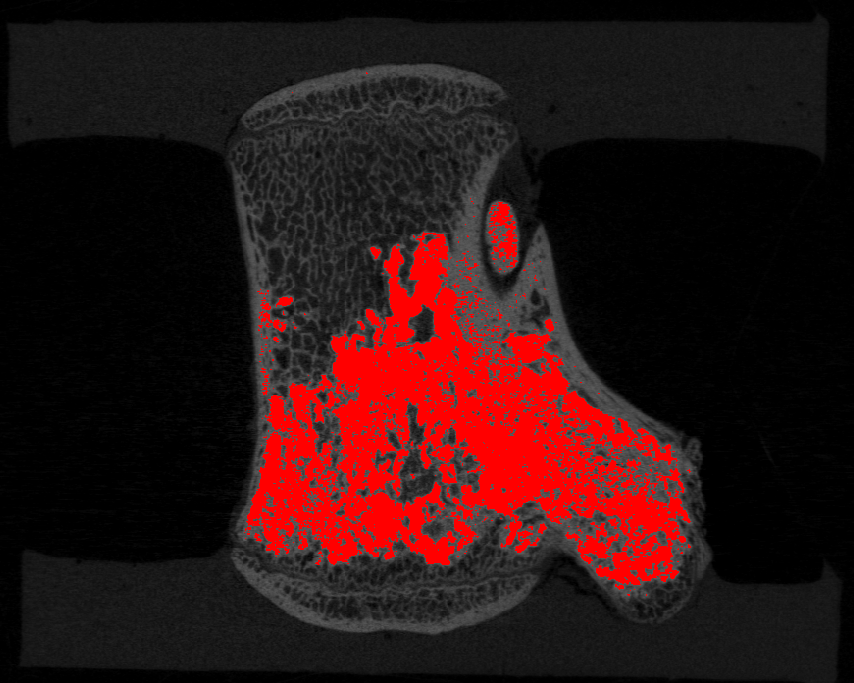
\includegraphics[width=10cm]{images/fullres_VP_segment.png}
  \caption{A lateral slice through an augmented bovine tail vertebra, showing
the cement mask in red.}
\label{fig:fullressVPseg}
\end{figure}


\subsection{Material Properties}\label{material-properties-bov}

\subsubsection{Bone Material Properties}

Material properties for the bone tissue were modelled elastically using a
bone element-specific elastic modulus (\(E_{\text{ele}})\) that is
dependent on the average greyscale value for the element in question
(\(\text{GS}_{\text{ele}})\) with the conversion factor between the two being $\alpha$.

\[E_{\text{ele}} = \alpha\ \text{GS}_{\text{ele}} (GPa)\]

This was required due to each element containing differing quantities of bone and bone marrow due to the continuum level modelling carried out. Hence, a homogenous value for the trabecular bone would not have represented the varying average of material properties seen in each element. Therefore, the conversion factor, $\alpha$ was used to convert between the greyscale value for each element and the Young's modulus.

This work was carried out in parallel to that described in the experimental sections above, however the experimental and computational methods remained the same. Specimens were divided into two groups of twelve  and were used to determine a conversion factor between greyscale and elastic modulus. This additional set of 24 specimens (separate to
those used in the above experimental study) was worked on in collaboration with Dr Sebastien Sikora, Dr Fernando Zapata Cornelio \& Ruth Coe (Research Fellow, Research Fellow \& PhD student respectively).
The groups consisted of a calibration group (used to determine the value of $\alpha$) and a validation group. For the validation group material properties were assigned - multiplying the greyscale
for each element by \(\alpha\) prior to compressing the model by 1 mm in
Abaqus and was used to validate against the experimental values of stiffness.

The calibration for \(\alpha\), the conversion factor was carried out
using a golden section search scalar optimisation process. Specifically
using the Brent method within the opti4Abq toolbox (Marlene Mengoni, University of Leeds). The objective of this toolbox was to find the root mean
square normalised difference between the experimental specimen stiffness
and the finite element stiffness and iterate until the objective
function achieved a value of 10\textsuperscript{-3}.

\subsubsection{Augmented Specimen Material
Properties}\label{augmented-specimen-material-properties}


For convenience the values for the Young's modulus for the interior cement volume were initially set to that of the inferior and superior end-caps. However, due to the rule of mixtures and the results found in the literature \cite{Kinzl2012a,Race2007}, the effect of reducing the Young's modulus was investigated. This was carried out by reducing the Young's modulus in 10 percent increments from a value of 2.45 GPa to 1.225 GPa.

Additionally, a preliminary investigation was carried out, identifying the effect of a yielding material interface between the bone and the cement, following the work by Sikora \cite{Sikora2013a}.
Here, a small interface layer (1 mm in thickness due to the model resolution) represents buckling that occurs in the trabeculae partially captured in the cement volume.
This investigation identified the effect of different yield stress values in combination with different Young's moduli for both the interface and the main cement volume.

The yielding region was created through the duplication and then erosion of the cement mask within Simpleware ScanIP, shown in \cref{fig:interfacecreation}.
This gave two masks, where one acts as the internal cement volume and the other as an interface layer.
Generic material properties were set to the region within ScanIP, allowing the values of the yield stress and Young's moduli values to be changed within the python setup script.

\begin{figure}[ht!]
\centering

	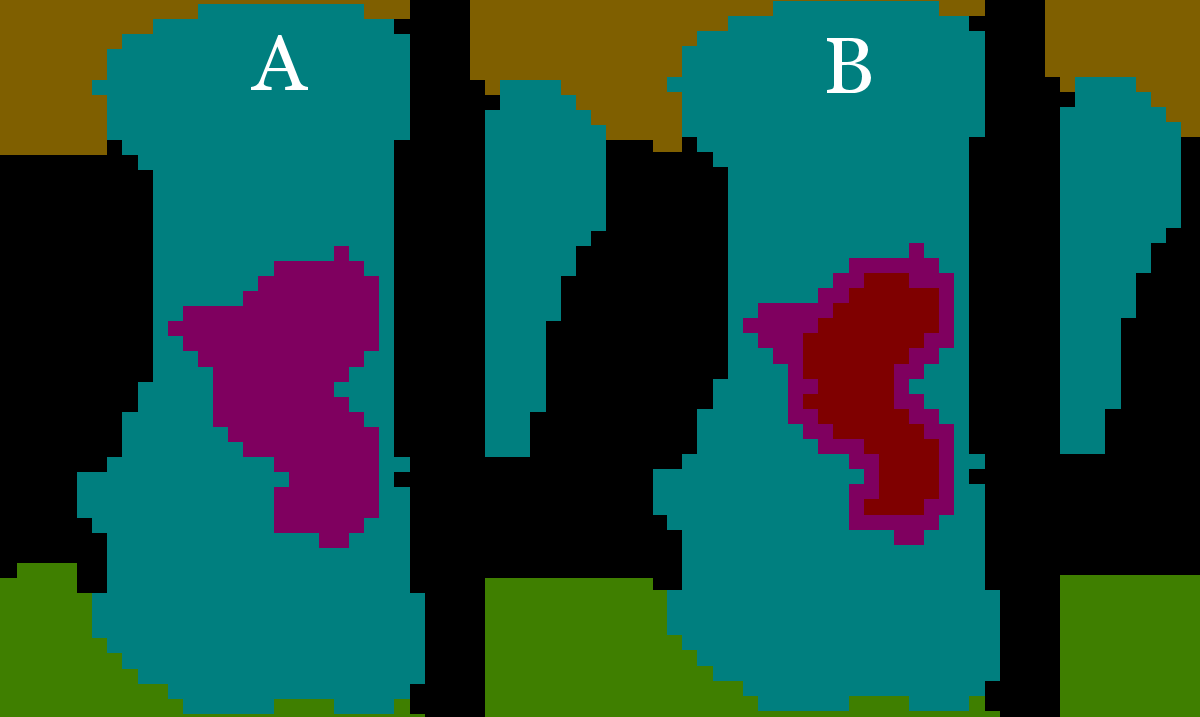
\includegraphics[width=10cm]{images/interface_creation.png}
  \caption{Creation of the interface layer: A, showing the initial description of the cement region in pink and B, showing the interface in pink and cement region in red, following the duplication and erosion.}
\label{fig:interfacecreation}
\end{figure}

\subsection{Sensitivity Tests}\label{sensitivity-tests}

\subsubsection{Mesh Size Sensitivity}\label{mesh-size-sensitivity}

Element sizes of 1 x 1 x 1 mm were used throughout, following previous
convergence studies on porcine vertebrae \cite{Jones2007}. The
results of the convergence study on porcine vertebrae showed that reducing the element
size below 2 x 2 x 2 mm led to changes in the model that were smaller
than predicted errors originating from other factors, such as
experimental errors and the simplification of boundary conditions.
However, reducing the element size to 1 x 1 x 1 mm allows greater
resolution when modelling the intricacies of the cement mesh for
augmented specimens, the difference between the two resolutions can be
seen in \cref{fig:vertslice}.

\begin{figure}[ht!]

\centering
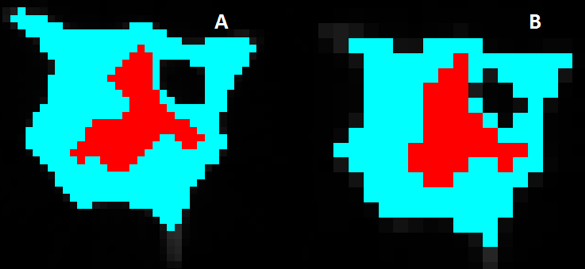
\includegraphics[width=3.90994in,height=1.80208in]{images/res_comp.png}
\caption{Mid-slice through an augmented vertebra, cyan: vertebral body, red:
cement. A, element size of 1 x 1 x 1 mm. B, element size of 2 x 2 x
2 mm.}
\label{fig:vertslice}
\end{figure}


\subsubsection{Sensitivity to an Additional
Mask}\label{sensitivity-to-an-additional-mask}

The addition of cement into the vertebral body created an extra mesh boundary
within the mesh containing the vertebral elements. In order to test what
effect this may have on the stiffness of models containing an extra
mesh boundary, an un-augmented specimen was tested with an extra mesh
representing the cement, but with the material properties of its
elements set based on their greyscale as with the other bone elements.
The mask was created by duplicating the vertebral mask and eroding it
until the volume was approximately 20 \% of its original volume. This
allowed testing to be carried out on the effect of the extra mesh alone,
while using an augmented specimen would allow a more accurate cement
shape, it would hinder setting material properties to that of the bone
greyscale and create an additional level of uncertainty. Mesh
interactions between the two meshes (internal vertebral surface and the
cement mask surface) were set using the contact pair interaction and
treated similarly to the interaction between the end-caps and the
vertebrae. Following model setup in ABAQUS as outlined in section \ref{model-creation} the model
was loaded in compression to 1 mm and its stiffness was recorded.

There was no difference between the two models, with and without the
internal cement mesh, meaning that any changes to the augmented model
stiffness was due to the material properties of the cement.

\subsubsection{Mesh Interactions}\label{mesh-interactions}

The effect of mesh interaction between the vertebral body and the
internal cement mesh were tested by comparing a) tied interactions
between the two surfaces and b) removing any interaction and merely
changing the material properties of the internal cement region
(neglecting the contact pair steps described earlier). This was carried
out for four augmented specimens following the same setup within ABAQUS
as described earlier.

The results can be seen in \cref{tab:meshint}, showing a negligible
difference
between variations for the four vertebrae models. This difference falls
well below the difference between experimental and computation,
especially for the augmented specimens, hence the effect of this
interaction can be neglected from further test.

\begin{table}[ht!]

\caption{The difference between interaction properties, tied and not tied for
four augmented vertebrae specimens.}
\label{tab:meshint}
\centering
%\resizebox{\textwidth}{!}{
  \begin{tabular}{c|c|c|c}
Vertebrae (Tail Number,  & Tied Interaction  & No Tied Interaction  &
Difference \\
Vertebral Level) & (N/mm) & (N/mm) & (\%) \\
\hline
\hline

T2 CC1 &	 5496 &	 5496 &	 0\\
T2 CC2 &	 8086 &	 8086 &	 0.001\\
T6 CC1 &	 3686 &	 3686 &	 0.001\\
T4 CC3 &	 6059 &	 6059 &	 0.0005\\ \hline

\end{tabular}
%}
\end{table}



\subsubsection{Augmentation Volume \& Location Sensitivity}

Another preliminary study was carried out into the sensitivity of the models to the position of the cement volume.
Tests were carried out to identify the effect of moving a 12 \% fill cement volume axially and sagittally in 2 mm increments.
This utilised the yielding interface described in \cref{augmented-specimen-material-properties} along with the +CAD tools built into Simpleware ScanIP to move a surface based description of the cement volume in the two anatomical planes.
A sphere surface of volume equivalent to 12 \% fill volume for the T12 CC2 vertebra was created within the +CAD software and imported into the project file for the vertebra, where it was positioned in it's first position.
This first position was 1 mm from the top of the vertebral body, ensuring 1 mm of bone surrounded the sphere.
It was then converted into a mask, duplicated and eroded in the same method described in \cref{augmented-specimen-material-properties}, with appropriate material properties.
Following this the mesh was generated and the abaqus input file was exported.
The sphere surface was then moved 2 mm in the inferior direction, the previous masks deactivated and the process repeated through the use of a python script to carry out the operations until the bottom of the vertebra had been reached.
This was also carried out in the sagittal plane. 


\subsection{Result Analysis}

The statistical approach to quantifying the agreement between the computational results and the experimental results for the measured stiffness uses the concordance correlation coefficient (CCC).
CCC measures the agreement between two variables and is described by Lin \cite{lawrence1989concordance} as a method to evaluate reproducibility.
The CCC is calculated as:
\begin{equation*}
  CCC = \dfrac{2 \rho \sigma_x \sigma_y}{\sigma_x^2 + \sigma_y^2 + (\mu_x - \mu_y)^2}
 \end{equation*}
Where $\mu_x$ and $\mu_y$ are the means for the two variables and $\sigma_x^2$ and $\sigma_y^2$ are the corresponding population variances.
$\rho$ is the Pearson correlation coefficient between the two variables.
For $n$ independent pairs of samples:
\begin{equation*}
	CCC = \dfrac{2S_{12}}{S_1^2 + S_2^2 + (\bar{Y_1}-\bar{Y_2})^2}
\end{equation*}
Where,
\begin{equation*}
	\bar{Y_j} = \dfrac{1}{n} \sum_{i=1}^{n} Y_{ij},\ S_j^2 = \dfrac{1}{n} \sum_{i=1}^{n} (Y_{ij} - \bar{Y_j})^2,\ j = 1, 2;
\end{equation*}
and
\begin{equation*}
S_{12} = \dfrac{1}{n} \sum_{i=1}^{n} (Y_{i1} - \bar{Y_1})(Y_{i2} - \bar{Y_2})
\end{equation*}

Specifically, this quantifies the degree to which pairs sit on the $x=y$ line.
Departures from this perfect agreement line result in a $CCC < 1$ even in cases where the Pearson correlation coefficient would equal 1.
$CCC = 0$ corresponds to no agreement and a value of $-1$ would be perfect negative agreement.



\subsection{Results} \label{bov:results}

The optimisation process gave a value for the conversion factor of 0.012529, allowing conversion between greyscale values for elements and their elastic modulus. This value was used for the bone constituents of the intact and augmented vertebrae presented in \cref{fig:compvexpscatter}, which shows the agreement between the \textit{in vitro} and \textit{in silico} results for the specimen specific models. The agreement of intact vertebrae was considerably better, with a concordance
correlation coefficient (CCC) of 0.49 compared with 0.16 for the augmented vertebrae (\cref{tab:int}), with the value increasing to 0.60 if the uncharacteristically stiff T8-CC2 was removed.

\begin{figure}[ht]
\centering
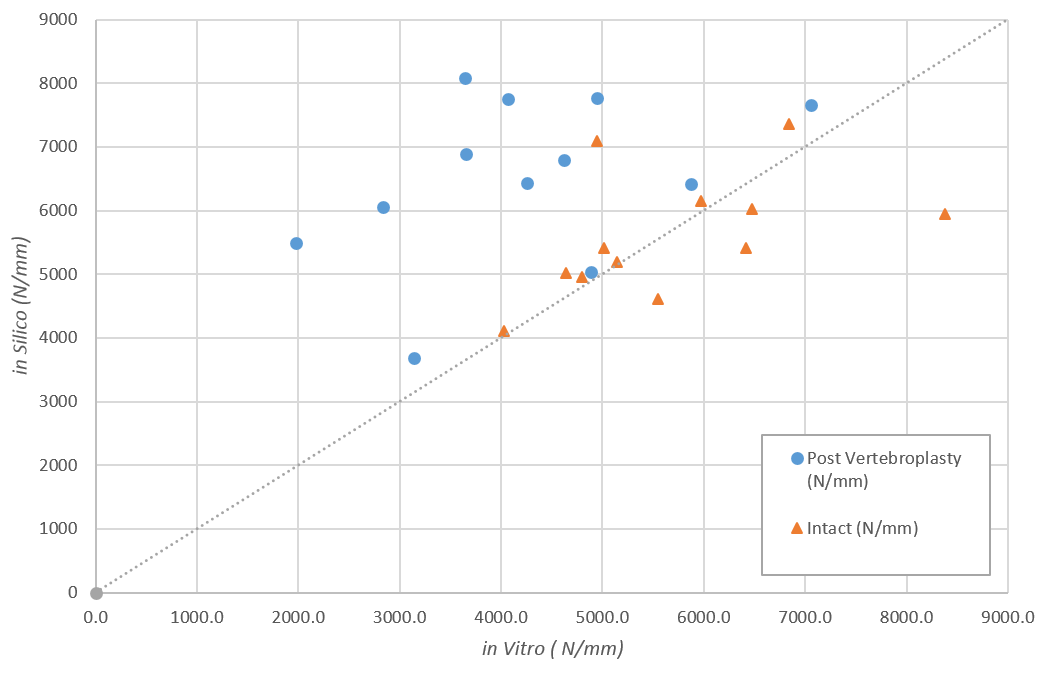
\includegraphics[width=\textwidth]{images/exp_vs_comp_both.png}
\caption{\textit{in silico} compared with \textit{in vitro} stiffness for intact specimens (triangles) and augmented specimens (circles). The dotted line shows a one-to-one correspondence.}
\label{fig:compvexpscatter}
\end{figure}

\begin{table}[ht]
\centering
\caption{The mean, standard deviation and concordance correlation coefficient (CCC) of the intact and augmented vertebrae for \textit{in vitro} and \textit{in silico results}.}
\label{tab:int}
\begin{tabular}{l|c|c|c}
     Intact Specimens     & Mean Stiffness & Standard Deviation & CCC                     \\ \hline \hline
\textit{in vitro}  & 5684 & 1196             & \multirow{2}{*}{0.4895} \\
\textit{in silico} & 5610 & 958               &                        \\
\hline
 Augmented Specimens
 \\ \hline \hline
\textit{in vitro}  & 4246 & 1371               & \multirow{2}{*}{0.1548} \\
\textit{in silico} & 6507 & 1298               &                      \\ \hline
\end{tabular}
\end{table}

The effect of changing the modulus of the cement volume in the augmented specimens is presented in \cref{fig:redEModBar}. There was a linear decreases in the stiffness of vertebrae with the reduction of he elastic modulus for the internal cement volume. The two vertebrae that show more prominent decreases in stiffness were those vertebrae that contained larger volumes of cement following their augmentation.

The effect that this has on the data with regard to the \textit{in vitro} stiffness results can be seen in \cref{fig:redEModscatter}, where the reduction in \textit{in silico} stiffness moves the data points closer to the $x = y$ line of perfect agreement between the experimental and computational results.


\begin{figure}[ht!]
\centering
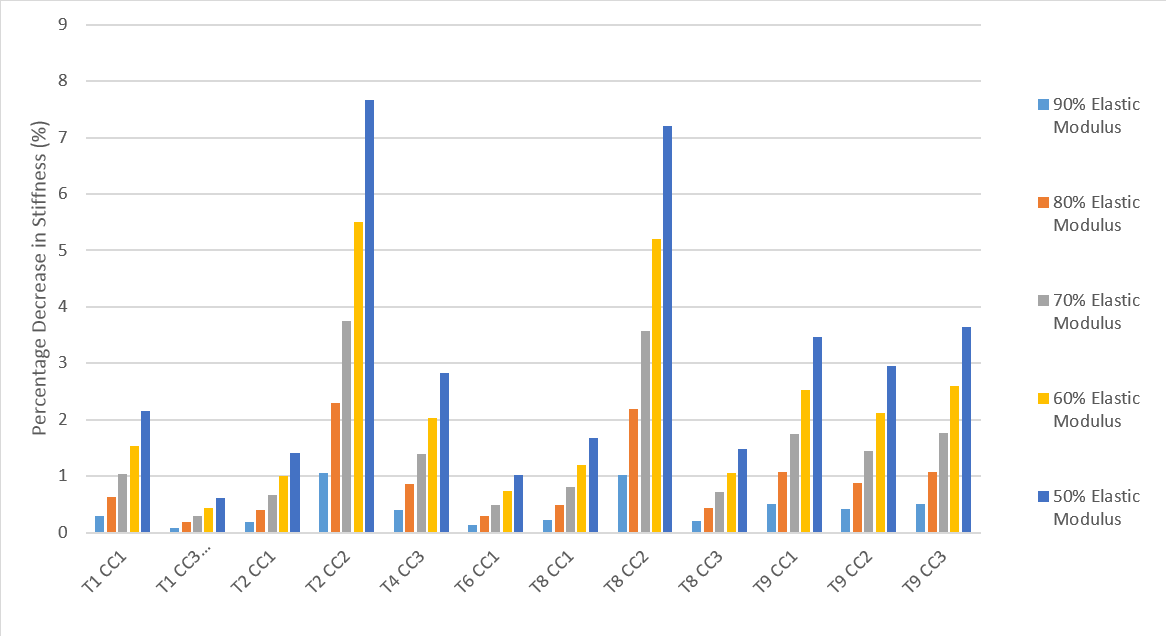
\includegraphics[width=\textwidth]{images/reductionOfEMod_Bar.png}
\caption{The percentage decrease in the vertebral stiffness after reducing the elastic modulus of the cement volume within 12 augmented vertebrae.}
\label{fig:redEModBar}
\end{figure}

\begin{figure}[ht!]
\centering
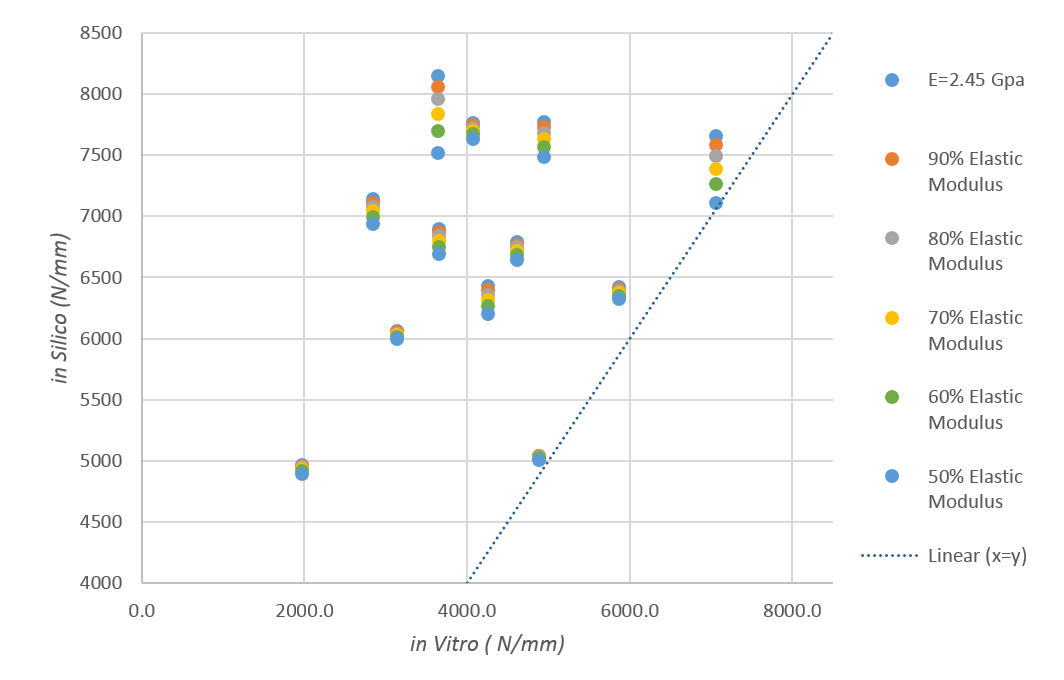
\includegraphics[width=5.3in]{images/reductionOfEMod_Scatter.png}
\caption{The effect of reducing the elastic modulus of the cement volume within 12 augmented vertebrae. Shows the in silico stiffness for the six elastic moduli tested against their in vitro stiffness. }
\label{fig:redEModscatter}
\end{figure}

\pagebreak

\subsection{Discussion}

The computational methods developed and results acquired, as with the experimental results, provide a good base for using human vertebrae and for the continued development of augmented vertebra modelling. The methods and automation of the creation of models both greatly reduce the time spent on model generation and reduce human error. This allows a relatively easy translation to human vertebrae, with only minor adjustments to the thresholds that define materials.

The current methods of masking and meshing the internal volumes of cement in the augmented models provides a good method of creating augmented models. The sensitivity tests carried out on the additional mask inside the vertebrae shows that any effects seen are due to the volume of cement and not a simulation problem. Similarly the inclusion of a tied interaction between the two meshes failed to affect the result, something especially useful when considering alternative mesh interaction to model the cement - trabeculae interaction.

The intact models agree well with experimental results, with very similar results for the mean and, excluding anomalous results, a good CCC value,  showing that the previously validated conversion factor works well with this set of data and that segmentation and model setup works correctly. The poor agreement with the augmented specimen models and their experimental counterparts was an expected result that agrees with similar studies in the literature - \cite{Wijayathunga2008}. In an attempt to
produce a better agreement, the elastic modulus of the cement volume was reduced in accordance with the experimental results of Race et al. \cite{Race2007} and similar methods employed by Wijayathunga et al. \cite{Wijayathunga2008}, where the reduction in modulus is expected due to the greater ratio of monomer to powder used, gaps between the bone and cement and pores within the cement. The reduction in stiffness forms a linear pattern as the elastic modulus is reduced, with those vertebrae that
show the greatest reduction being those containing the largest volume of cement. While these results do show a reduction in the stiffness, closer to that of the experimental values, it does not explain the disagreement fully. This suggests that a combination of improvements to the augmented models is required.

Future work will utilise the results acquired, especially those relating to the cement modulus and the cement - bone interactions, to understand how to model this interface more realistically and achieve good agreement between experimental and computation results of stiffness for augmented specimens.


